\chapter{Reconstruction}
\label{annex:detectors-sc-physics-software-reconstruction}

The raw data from the near and far detectors provide highly detailed views of neutrino
interactions and background events, which must be reduced and interpreted in order to
extract the physics measurements.  Cosmic rays must be identified and rejected, tracks and
showers selected, particle identities assigned to the reconstructed objects, and event-level
interpretations formed.  While the performance of the reconstruction in both the Near Detector
and the Far Detector have direct impacts on the physics sensitivity of the experiment, effects
resulting from the detector designs and the angular and momentum acceptance differences of the
near and far detectors are ingredients in the systematic uncertainty estimations that also
affect the sensitivity of the experiment.  If a particular class of events has a different
reconstruction efficiency or energy resolution in the near and the far detectors, then modeling of the fraction of events
in this class may become important, and cross sections and nuclear modeling systematic uncertainties
can enter in this way.  The fact that the near detector is smaller than the far detector and accepts a larger
angular range of particles from the beam will introduce some of the systematic uncertainties even if the
technologies are the same. 

\section{Near Detector Reconstruction}
\label{annex:detectors-sc-physics-software-reconstruction-nd}

\fixme{To be supplied, even if it is brief}

\section{Far Detector Reconstruction}
\label{annex:detectors-sc-physics-software-reconstruction-fd}

The reconstruction of particle interactions in Liquid Argon TPC
detectors is an active area of research and development.
A series of sophisticated reconstruction algorithms are required to
address a broad range of complex event topologies, and to perform
precise physics measurements that fully exploit the spatial and 
calorimetric precision offered by Liquid Argon technology.
Although the field is not yet mature, there has been considerable
progress in recent years, including the first fully automated
pattern recognition algorithms. 

A fully automated event reconstruction will be developed for the
DUNE Far Detector. The block diagram in Figure~\ref{fig:fdrecoblockdiag}
illustrates the components of the Far reconstruction chain. 
The first stage involves the processing of the noisy ADC wire signals,
and creation of 2D `hits'. A series of pattern recognition algorithms
are then used to group the hits into 2D and 3D clusters representing 
individual particle tracks and showers. A set of high-level tools
then reconstructs the vertex and 3D trajectory of each particle,
provides particle identification, and reconstructs the four-momentum.
While each step of the reconstruction chain has been implemented,
the algorithms have not yet been fully optimized.
\fixme{Not sure whether or not to mention LArSoft and Qscan explicitly here}
The following sections describe the current status of each task.

\begin{cdrfigure}[Far detector reconstruction block diagram]{fdrecoblockdiag}
{Block diagram showing the components of the far detector reconstruction chain}
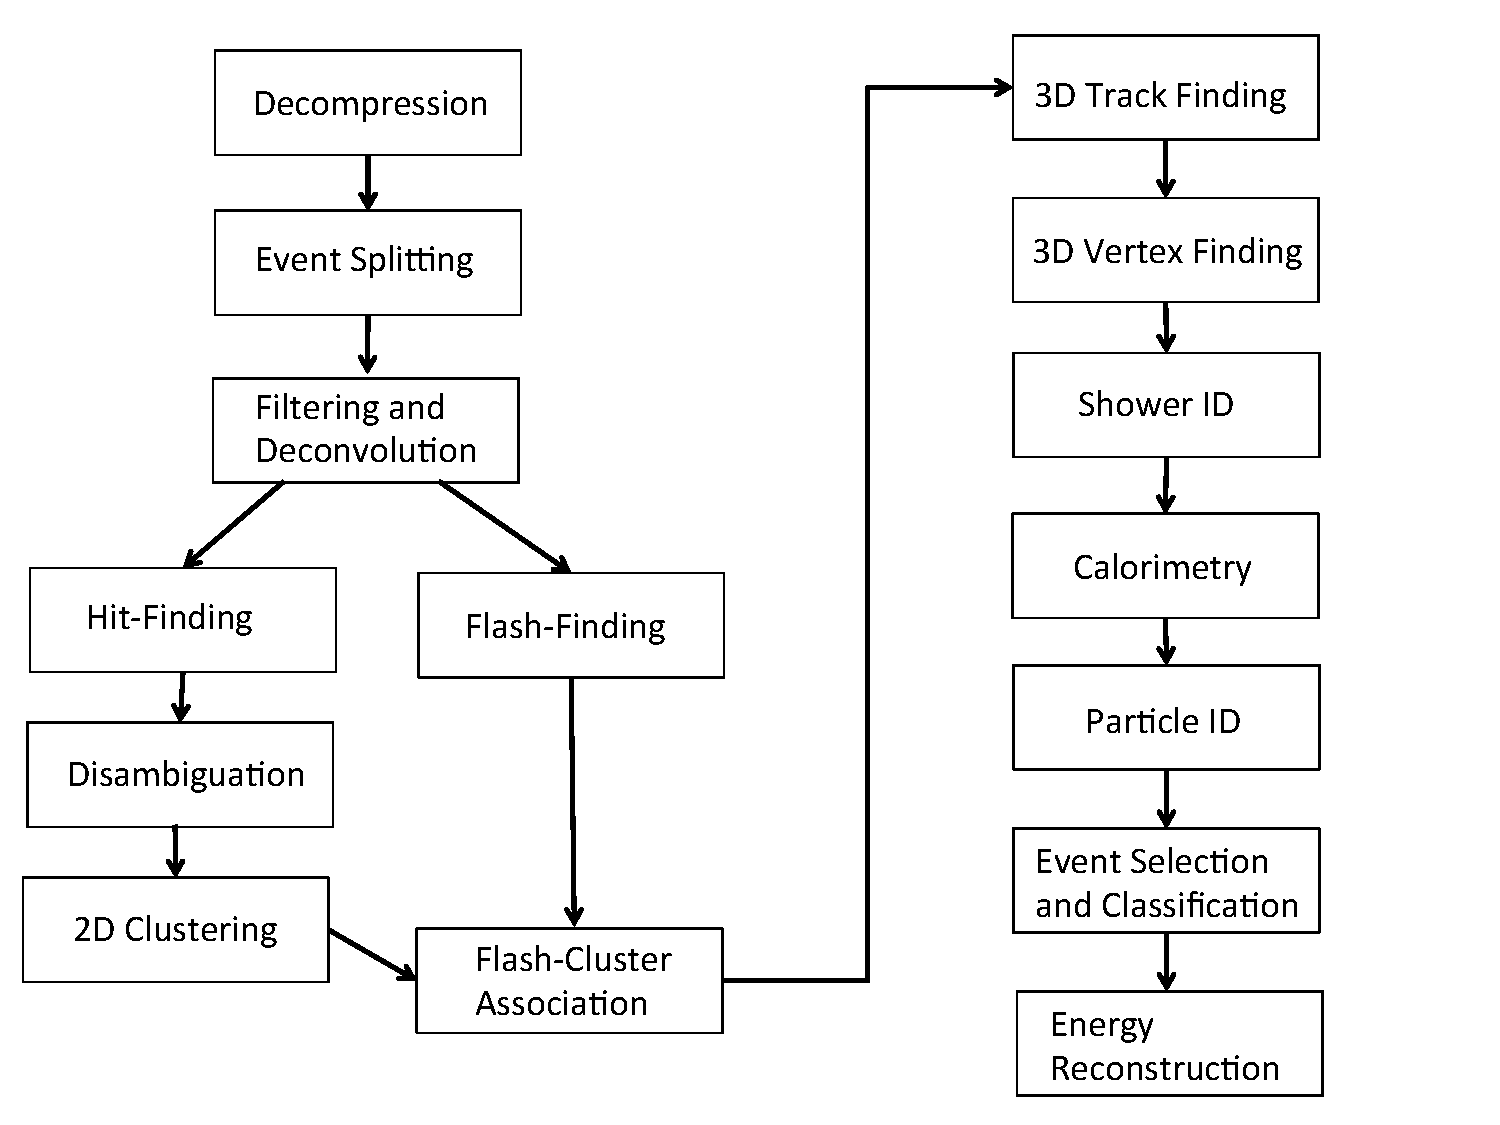
\includegraphics[width=0.8\textwidth]{fdrecoflowchart_annex.pdf}
\end{cdrfigure}

\subsection{Signal Processing and Filtering}

A series of signal processing algorithms have been developed to
perform noise reduction and baseline subtraction on the digital
waveforms read out by Liquid Argon TPC detectors. 
These algorithms have been validated on data from 
\fixme{say where...}.

The TPC data are first uncompressed and put into local storage, one channel at a time.  
In the case that the DAQ writes data records to persistent
storage the correspond to inconveniently long time periods, the data may be split
into smaller events at the readin stage.  At this stage, if an interaction is found
to have taken place near the edge of the time corresponding to one record from the DAQ,
the next one may be appended to make an offline event that corresponds more closely to
what is required to analyze the interaction of interest.

\subsubsection{Single-Phase Signal Processing and Filtering}

The detector response (bipolar vs. unipolar), and
electronics response functions are deconvoluted using a Fast Fourier
Transform (FFT) algorithm.  The FFT of the data are multiplied by the
inverse of the convolution kernel used in the simulation process,
multiplied by the frequency response of a noise filter, which
suppresses low-frequency and high-frequency noise.  It may be
necessary to filter unipolar signal components on the induction-plane
wires and handle these signals separately, in the case of partial
non-transparency of the induction planes, which might be unavoidable
near the wrapping boundaries.  The product of these is then
inverse-FFT'd back to the time domain to yield the deconvoluted
signals.  A computational speedup is achieved by packing data in
blocks that exceed thresholds plus nearby neighbors in time so that
the FFT only needs to see a fraction of the total ADC samples
collected in each event.

\subsubsection{Dual-Phase Signal Processing and Filtering}

Qscan also provides a set of methods for signal processing. 
The raw waveforms are first processed: this involves noise reduction as well as the subtraction of the baseline.
Hits, defined as signals that are discriminated from the noise, are identified and reconstructed.
In order to suppress noise without affecting the signal component too much, hence improving the signal to noise ratio, 
two different algorithms are used: the Fast Fourier Transform (FFT) filter, and the coherent noise subtraction algorithm.
A smooth cut-off, implemented with a Fermi potential, efficiently suppresses the noise without introducing artifacts in the
time domain.
The coherent noise filter is implemented to remove identical noise patterns that are seen on larger sets of readout channels. 
Unlike in the case of the FFT filter, which directly suppresses the frequencies of single 
channels and thus reducing the signal bandwidth, the coherent noise filter ideally subtracts only the noise while keeping the signals unchanged.
After suppressing the noise, the (constant) pedestal of each waveform has to be computed and subtracted from each sample.

\subsection{TPC Hit Finding}

Once deconvoluted, raw ADC values trace out pulses, which are the best
estimates of when charge arrived on a particular electronics channel.
The widths of these pulses are determined by the detector resolution,
by diffusion, and by the intrinsic width of the charge formation
volume projected along the electric field dirction, which can be quite
long in the case of showers or tracks nearly aligned with the electric
field.  Multiple particles may contribute charge to the same pulse,
which is expected to be the case frequently in dense electromagnetic
showers, but can also occur from different particles leaving charge on
segments of the wire that are far apart, as the data from a wire do
not tell where along the wire the charge was deposited.  
Due to the wrapping of the induction-plane wires, pulses can contain charge
from opposite sides of the APA, but not for collection-plane signals.

\subsubsection{Single-Phase Hit Finding}

Hits are reconstructed pulses on each TPC DAQ channel.  Regions of
interest are identified in the stream of deconvoluted ADC samples, and
sums of Gaussian functions are fitted to the data using
MINUIT~\cite{James:1994vla}.  The peak position, the width, the area, and the
sum of the deconvoluted ADC values corresponding to the fitted
Gaussian are recorded.  In the case that multiple overlapping Gaussian
fits are the best model of the data, the ADC sums are calculated for
the entire region of interest, and then divided among the contributing
hits proportional to their fit areas.  

\fixme{Hit-finder performance plot?}

%The efficiency of the hit
%finder is shown in Figure~\ref{fig:hitfinderefficiency}.

\subsubsection{Dual-Phase Hit Finding}

In Qscan, hits have to be extracted from the signal waveforms by means of a standard threshold discrimination. 
Due to changing noise conditions, the threshold is defined in relation to the measured RMS noise value, 
which is measured for each event and readout strip, using the pre-trigger samples.
In the general case there can be several close or overlapping tracks per event, producing a superposition of several signals/hits on a single readout strip. 
The shaping time constants of the preamplifiers are chosen such that double tracks being separated by a few $\mu s$ can be resolved.
The hit finding algorithms therefore extract multiple hit information by fitting the waveform function of the signal.
The main parameters determined for the fitted hits are the hit time and the hit integral: 
together with the location of the corresponding readout channel, the hit time directly provides the information of the hit location in the considered view (projection), whereas the hit integral is related to the produced ionization charge and therefore provides the calorimetric information.


\subsubsection{Single-Phase Disambiguation}

A feature of liquid argon TPC geometries is that the location along a
wire at which charge is deposited is not measured, creating a
one-dimensional continuous ambiguity in the interpretation of the hits
on a wire.  As such, the planes of the TPC read out two-dimensional
``views'' of the three-dimensional events.  The wrapping of the
induction-plane wires in the DUNE APA design introduces another
discrete ambiguity -- the several wire segments that are connected
together to form a DAQ channel all contribute charge on that DAQ
channel, and it is not known from the wire's signal which of those
segments generated the charge.  This discrete ambiguity must be broken
before downstream reconstruction programs can do their work.

The detector geometry is chosen so that no induction-plane wire
crosses any collection-plane wire more than once, necessitating a
shallower induction-plane wire angle of 35.7$^\circ$.  The design from
the LBNE CDR~\cite{lbnecdr} proposed 44.3$^\circ$ and 45.7$^\circ$ as
the angles of the $U$ and $V$ wire planes, which necessitated
associating triplets of $U$, $V$, and $Z$ hits in order to break the
ambiguity.  Hit triplets consistent in drift time and with only one
possible combination of $U$, $V$, and $Z$ hits that intersect in one
position in space are determined to be ``trivially'' disambiguated.
More complicated cases where multiple possible hits in other planes
can be associated with a hit in a given plane, are disambiguated by
looking at nearby unambiguous hits and clustering them together.
Misassociation of hits in the three views, caused mainly by multiple
charge deposits arriving at the same time, can cause choosing the
incorrect wire segment.

The triplet-association algorithm is expected to work very well in the
35.7$^\circ$ geometry, by making few misassociations for the trivially
disambiguated sample.  Figure~\ref{fig:disambig_annex} shows the
disambiguation performance for 6~GeV electrons and muons in the
35.7$^\circ$ far detector geometry.  The algorithm used was developed for 35-ton event
reconstruction, and has not yet been optimized for the 35.7$^\circ$ far detector geometry.
Nonetheless, the performance is quite good, with a negligible fraction of mis-disambiguated hits,
while the fraction of un-disambiguated hits can be lowered by improving the clustering step.
A change request was granted in 2014 to
move from the 44.3$^\circ$, 45.7$^\circ$ wire angles to the shallower angle
of 35.7$^\circ$ in order to improve the expected disambiguation performance.

\begin{cdrfigure}[Disambiguation performance]{disambig_annex}
{Simulated performance of the 35-ton disambiguation algorithm applied to the single-phase Far Detector
design, for 6~GeV electrons and muons, shown separately as functions of the angle of the initial particle
with respect to the plane parallel to the anode wires.  The black curve shows the fraction of hits that
are correctly disambiguated, the red curve shows the fraction of hits that are assigned the wrong wire segment,
and the blue curve shows the fraction of hits that remain ambiguous, to be addressed by optimizing the algorithm.}
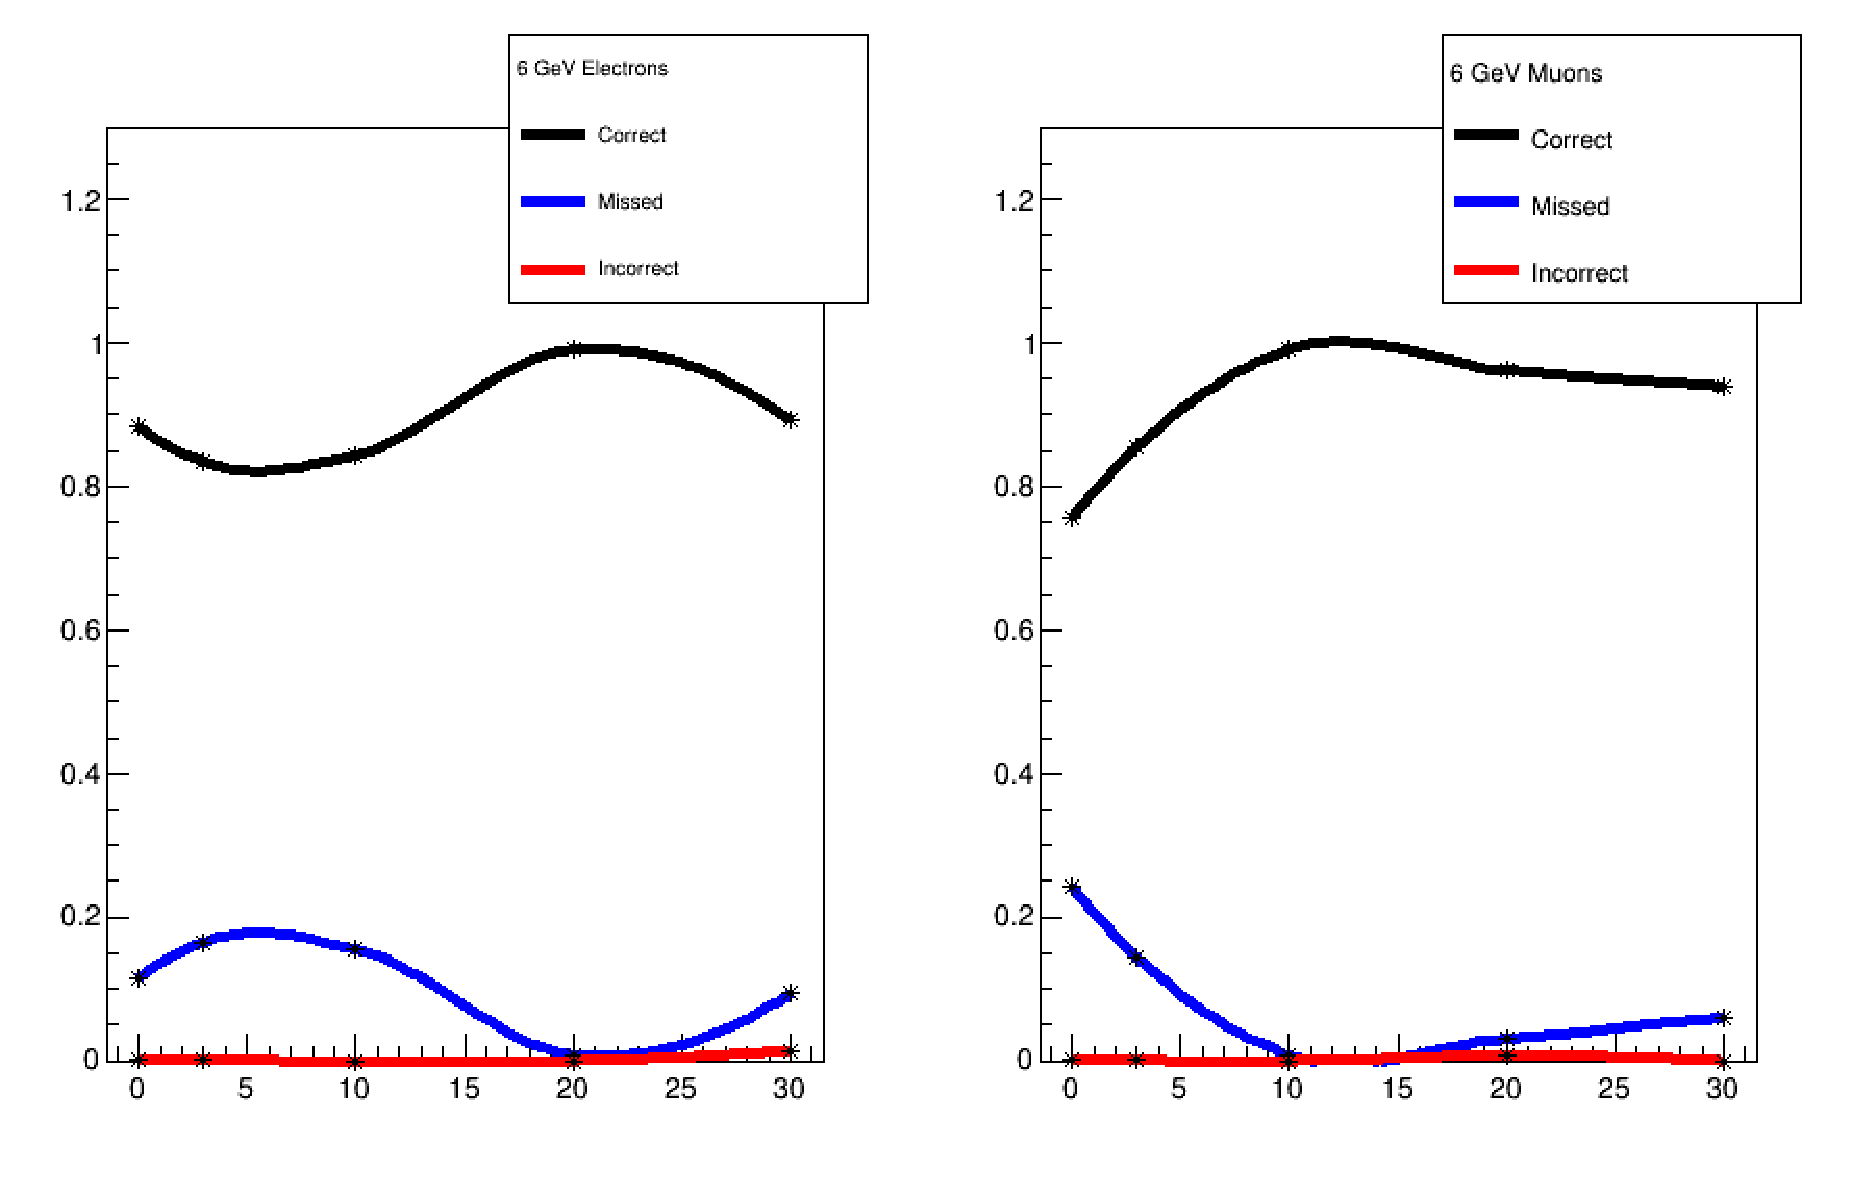
\includegraphics[width=0.8\textwidth]{disambigfractions_36.pdf}
\end{cdrfigure}

\subsection{Optical Detector Signal Reconstruction}

The optical detector signals are reconstructed in two steps.  First, a
hit finder identifies signals on an individual channel, looking for
peaks while account for noise and pedestal.  Each hit is assigned a
total integrated charge and a time associated with the first peak,
since the SiPM signals are asymmetric and multiple individual photons
may get grouped together into a single hit if they are close in time.
Second, a flash finder groups together hits from across multiple
photon detectors which are coincident in time (a ``flash'' being a
source of light in the detector like the scintillation from the
passage of a charged particle).  Each flash has a total integrated
charge determined from its constituent hits as well as a
two-dimensional position determined by a charge-weighted average of
the positions of the photon detectors.  Since the photon detectors all
sit in a single plane, only two dimensional position reconstruction is
possible.  Once a flash is reconstructed, it becomes a candidate $t_0$
for objects reconstructed by the TPC.  If only a single track or
shower is present in the detector near the time of the flash, the
association is clear, but if there are multiple overlapping tracks a
likelihood-based method associates a TPC object with its best matching
flash.


\subsection{TPC Hit Clustering}

After the hit-finding and disambiguation stages have completed, a series of 
pattern recognition algorithms are applied to the 2D hits in order to identify 
the tracks and showers produced by individual final-state particles in an event.
In Liquid Argon TPC detectors, the pattern recognition stage must perform 
two functions in order to reconstruct 3D particles from 2D hits:
(a) identify the patterns of hits within each two-dimensional view
that correspond to individual particles; (b) match up hits and trajectories
between views in order to reconstruct particles as three-dimensional objects.
The development of automated pattern recognition algorithms for Liquid Argon 
TPC detectors is a relatively new field, but several 2D and 3D algorithms
have been implemented, using a range of different techniques.
For example, the ``Fuzzy Cluster'' package is a suite of algorithms that
performs two-dimensional clustering of hits using several techniques developed 
outside of HEP~\cite{flameclustering}~\cite{pphtclustering}~\cite{Ester96adensity-based}.

A promising suite of pattern recognition algorithms, that provides fully 
automated reconstruction of 3D particle tracks and showers from 2D hits, 
is the PANDORA software development kit~\cite{Marshall:2013bda,Marshall:2012hh}.
PANDORA implements a highly modular approach to pattern recognition,
in which the final-state particles within an event are reconstructed using 
a large chain of focused algorithms, each designed to identify and handle
a specific event topology. The reconstruction chain begins with a 
series of 2D pattern recognition algorithms that group together hits 
into clusters based on their topology and spatial proximity.
The next stage of the chain is 3D track reconstruction, 
which uses a rank-three tensor to match up all possible combinations 
of 2D clusters between the $U$, $V$, and $Z$views, and group together 
the best-matched triplets or doublets of clusters. If necessary, 
2D clusters are modified to improve the consistency of the 3D event. 
Once the 3D track trajectories have been identified, 
a series of vertex-finding algorithms are applied to the event,
which reconstruct the neutrino interaction vertex by analyzing 
the 2D and 3D event topology. The remaining 2D clusters are then
used to reconstruct electromagnetic and hadronic showers,
first as extended 2D clusters, and then as 3D particles, 
using a similar procedure to 3D track reconstruction.
Finally, a neutrino event is formed by connecting together the 
reconstructed tracks and showers at the interaction vertex.

\fixme{In the single-phase reconstruction, the availability of 
three views provides strong constraints on 3D ambiguities}

Figure~\ref{fig:recoannexpandoraeventdisplays} shows some event displays....

The PANDORA pattern recognition algorithms have been developed
using simulated neutrino interactions in the energy range 100\,MeV\,$-$\,25\,GeV.
Figure~\ref{fig:recoannexpandoraefficiency} shows the efficiency for reconstructing
the leading final-state lepton in 5\,GeV $\nu_{e}$ CC and $\nu_{\mu}$ CC interactions,
plotted as a function of momentum using the MicroBooNE detector geometry.
In both samples, the reconstruction efficiency increases rapidly with momentum,
rising above 90\% at 500\,MeV and reaching approximately 100\% at 2\,GeV.
Figure~\ref{fig:recoannexpandoravertexresolution} shows the spatial resolution for
reconstructing the primary interaction vertex in 5\,GeV $\nu_{\mu}$ CC events,
projected onto the $x$, $y$ and $z$ axes. An estimate of the overall vertex 
resolution is obtained by taking the 68\% quantile of 3D vertex residuals, 
which yields 2.2\,cm (2.5\,cm) for $\nu_{\mu}$ CC ($\nu_{e}$ CC) events.


\fixme{CLUSTERING/PANADORA FOR LBNO (TWO VIEWS), taken from LGUNA-LBNO deliverables51 }

Algorithms specific for two views event reconstruction have been extensively developed as well. 
A preliminary 2D clustering is carried on similarly to what described above.
A first-pass hit clustering, using a nearest-neighbor algorithm and association algorithms is performed
on each projection. Then primary vertex is found based on presumed beam direction and cluster positions/directions
(redundant information from all readout views is used to constrain the vertex location).
Primary final-state particles (seed-clusters) are finally identified, based on cluster length and proximity to vertex,
and each of the remanining non-seed cluster is associated with existing seed-clusters so that all energy deposits from a single final-state particle are grouped together.
At the end of this process, clusters not directly related to the vertex (either by pointing or position) 
will be associated with clusters coming from the vertex which are in close proximity, 
as long as there is not another vertex-related cluster nearby. 
%Any remaining clusters far from the vertex will be removed, 
%since it is assumed that these are actually related to an original final state particle, but we have been unable to make the association.

The PANDORA reconstruction has been tested on charged current events generated by both   $\nu_{e}$  and $\nu_{\mu}$  
considering the processes $\nu_{\ell}\to \ell+p$  and $\nu_{\ell}\to \ell+p+\pi^{+}$.
Neutrino energy distribution is simulated by means of a detailed beam flux simulation.
Final state neutrino interaction particles were then generated by taking GENIE output, selecting only events with matching final state topologies, 
and simulating these events using Qscan.
 The performance has been tested by using truth information to associate each final state particle with up to one reconstructed cluster.
The quality of the reconstruction of each final state particle is then evaluated by calculating the ``completeness'' and purity for each particle.
The former is defined as the proportion of the true particle energy deposit which 
is contained in the associated cluster, the latter as  the proportion of the associated cluster energy which was actually deposited by the final state particle.
Both completeness and purity is above 90$\%$ for particles energy above above 800 MeV, while
it is seen that cases of poor reconstruction are largely due to lower-energy particles which are more difficult to identify.

\fixme{Overflow from CDR:}

For the dual-phase event reconstruction, where only two views are available,
the PANDORA reconstruction uses a similar set of 2D algorithms but
a modified 3D approach. The quality of the neutrino event reconstruction 
is evalulated by performing hit-by-hit comparisons of simulated and 
reconstructed particles and calculating the following performance metrics: 
``completeness'' is defined as the fraction of hits generated by 
the true particle and contained in the reconstructed particle; 
``purity'' is defined as the fraction of hits in the reconstructed 
particle that were deposited by the true particle. 
Both the completeness and purity are found to be above 90$\%$ for 
final-state particles with energies above 800\,MeV.

Figure~\ref{fig:recoannexpandoraperformancemetrics} shows purity and completeness metrics ...




\begin{cdrfigure}[PANDORA event displays]{recoannexpandoraeventdisplays}
{CAPTION GOES HERE}
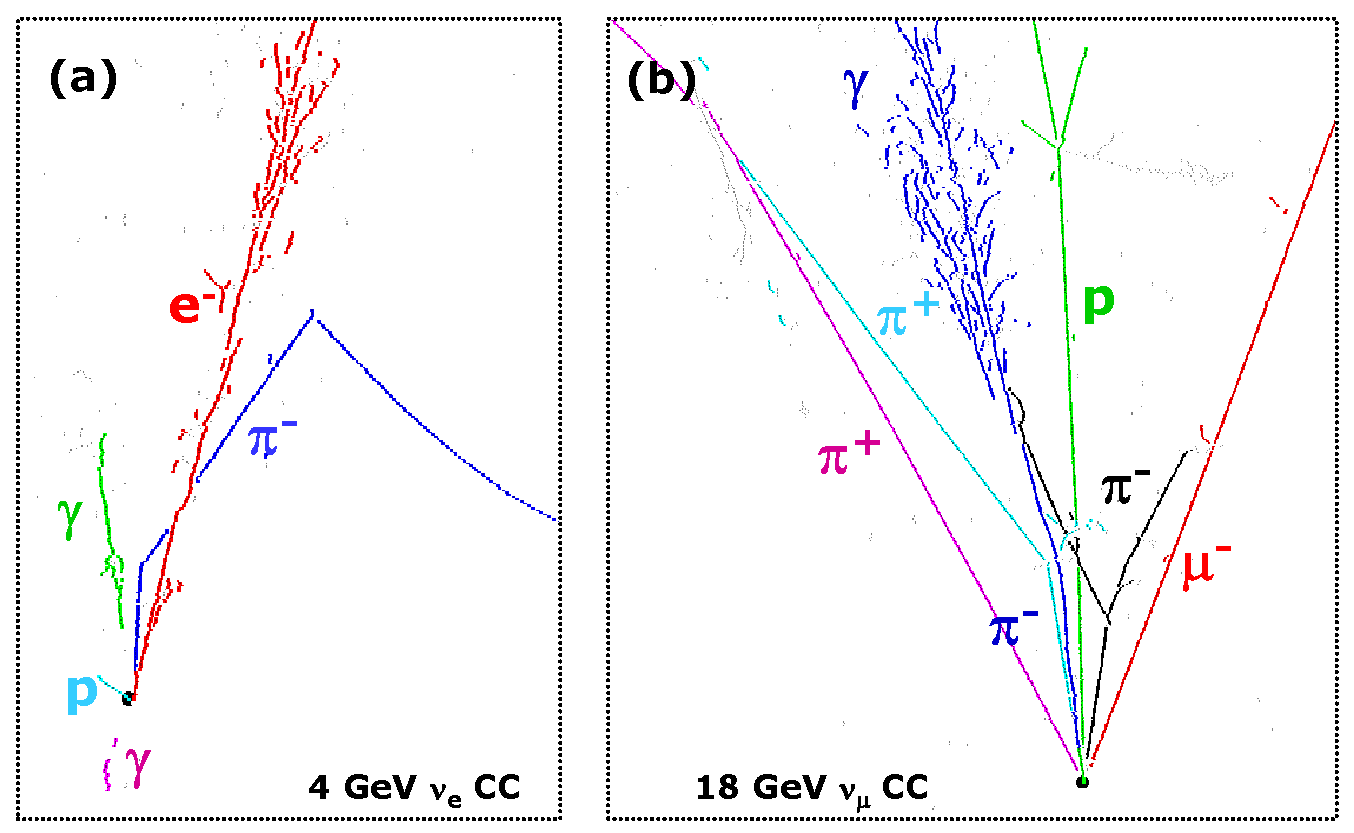
\includegraphics[width=\textwidth]{LArReco_EventDisplays_Take3.pdf}
\end{cdrfigure}

\begin{cdrfigure}[PANDORA reconstruction efficiency]{recoannexpandoraefficiency}
{Reconstruction efficiency of Pandora pattern recognition algorithms
 for the leading final-state lepton in 5\,GeV $\nu_{\mu}$ CC (left) and
 $\nu_{e}$ CC (right) neutrino interactions, plotted as a function of
 the lepton momentum. The reconstruction performance is evaluated
 using the MicroBooNE detector geometry. }
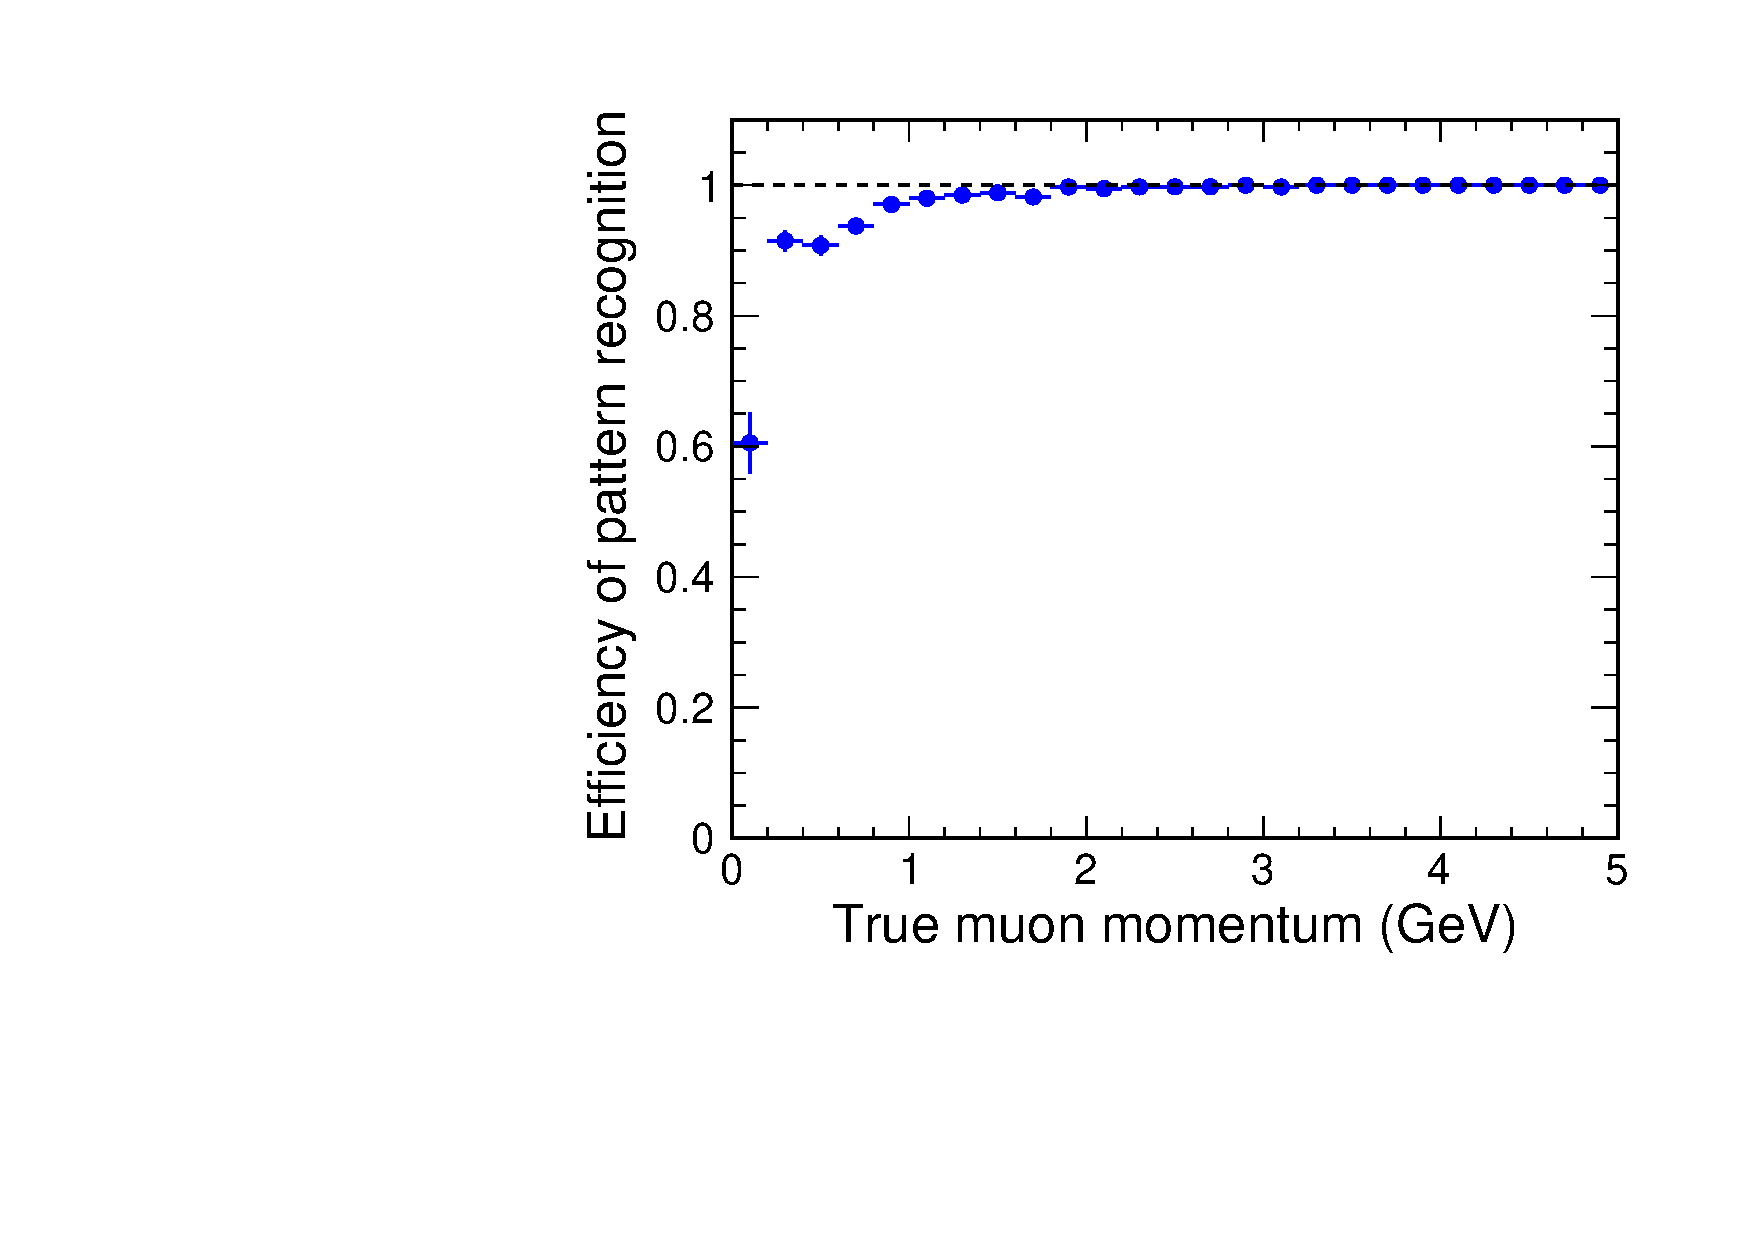
\includegraphics[width=0.49\textwidth]{pandora_uboone_efficiency_5GeV_numucc_annex.pdf}
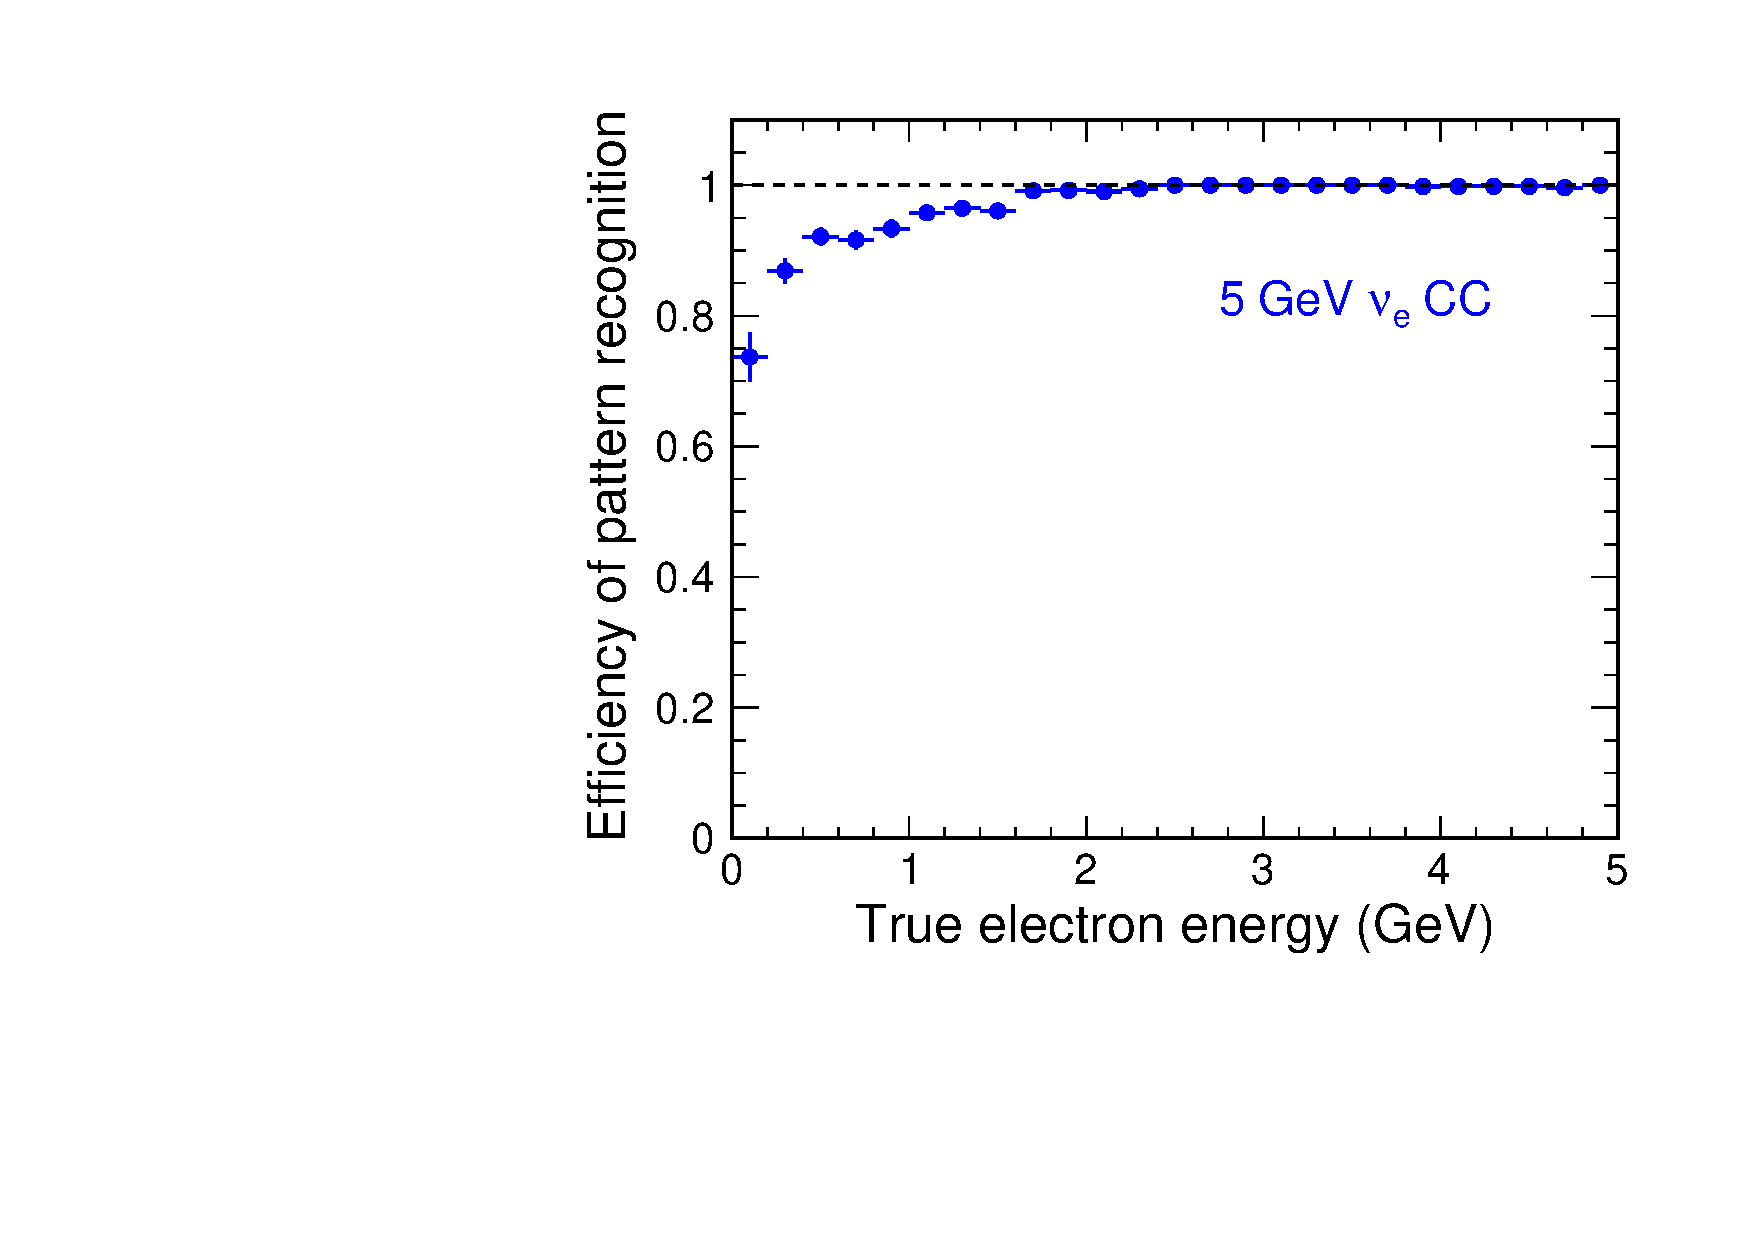
\includegraphics[width=0.49\textwidth]{pandora_uboone_efficiency_5GeV_nuecc_annex.pdf}
\end{cdrfigure}

\begin{cdrfigure}[PANDORA purity and completeness]{recoannexpandoraperformancemetrics}
{CAPTION GOES HERE}
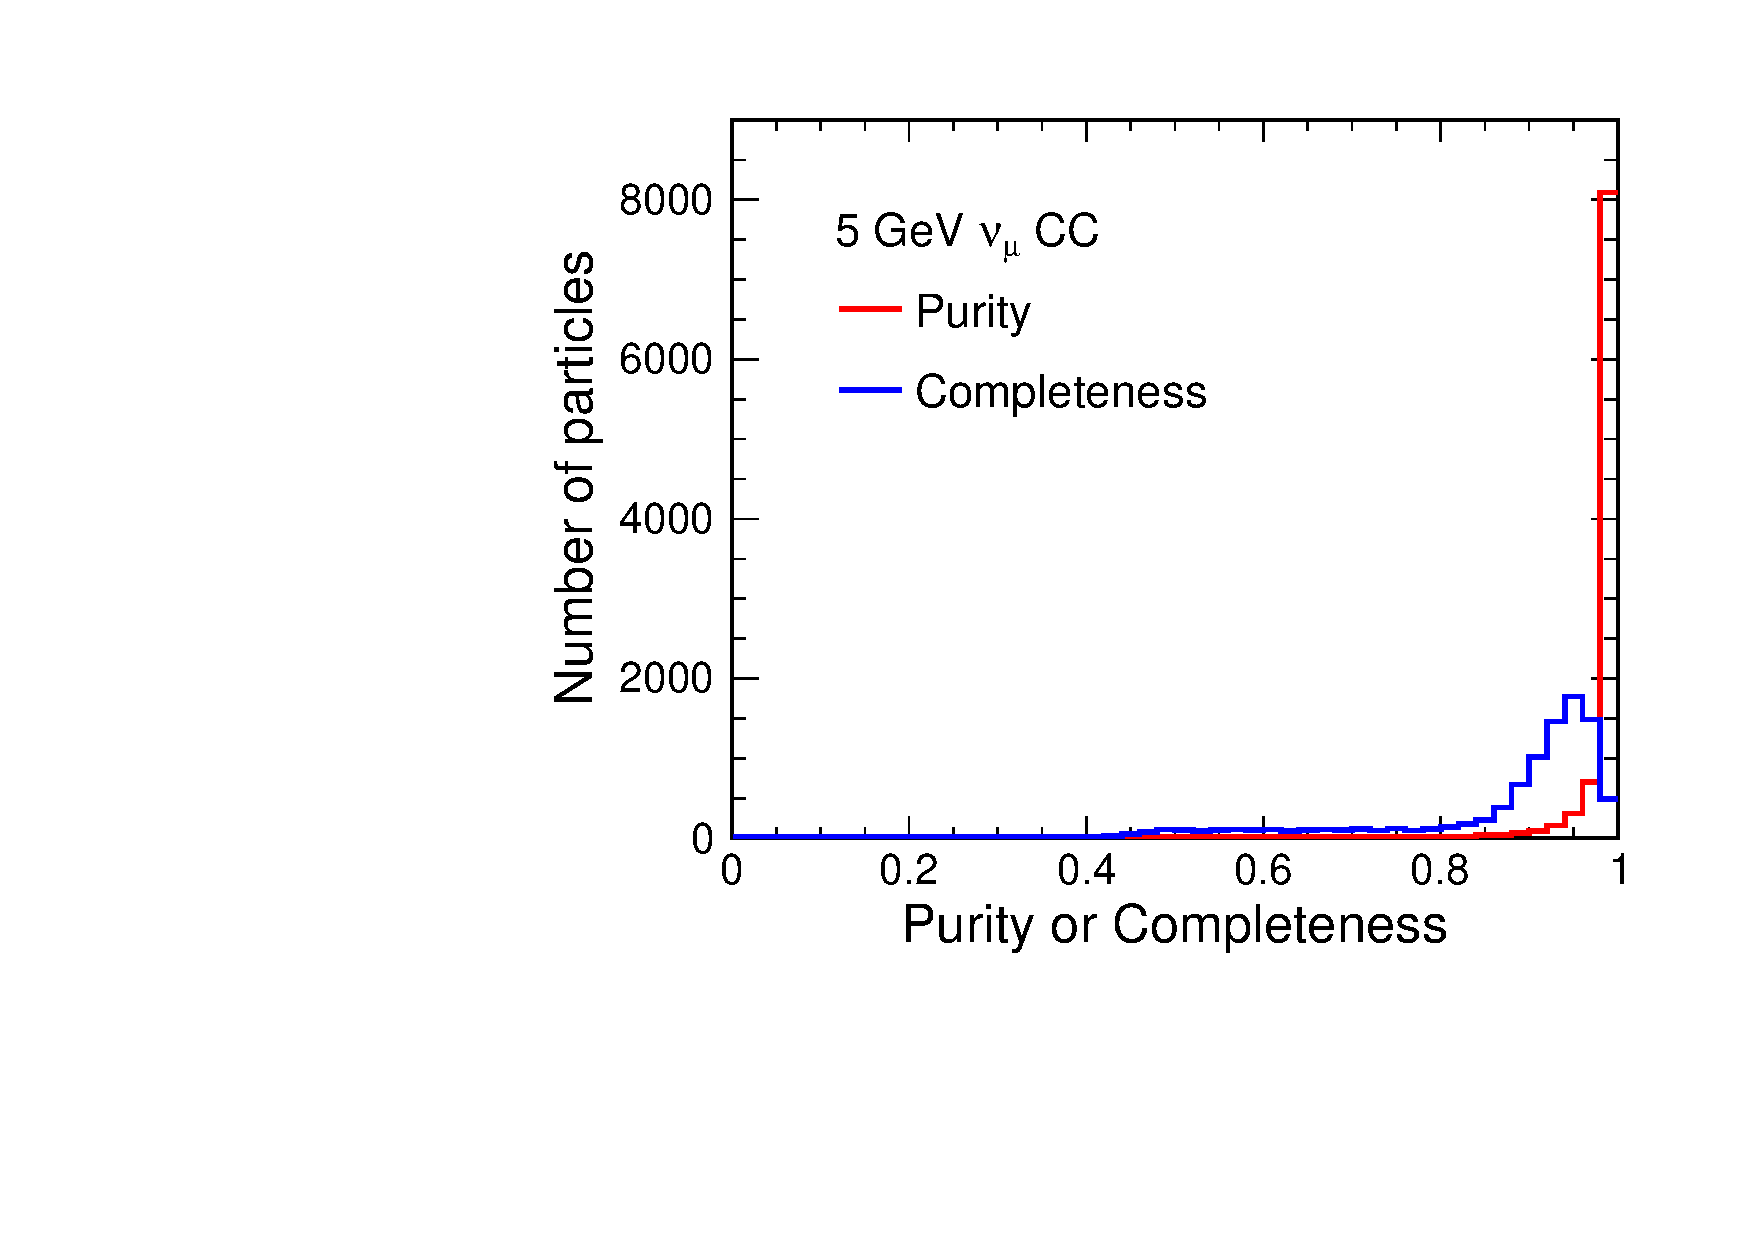
\includegraphics[width=0.49\textwidth]{pandora_uboone_purity_completeness_5GeV_numucc_annex.pdf}
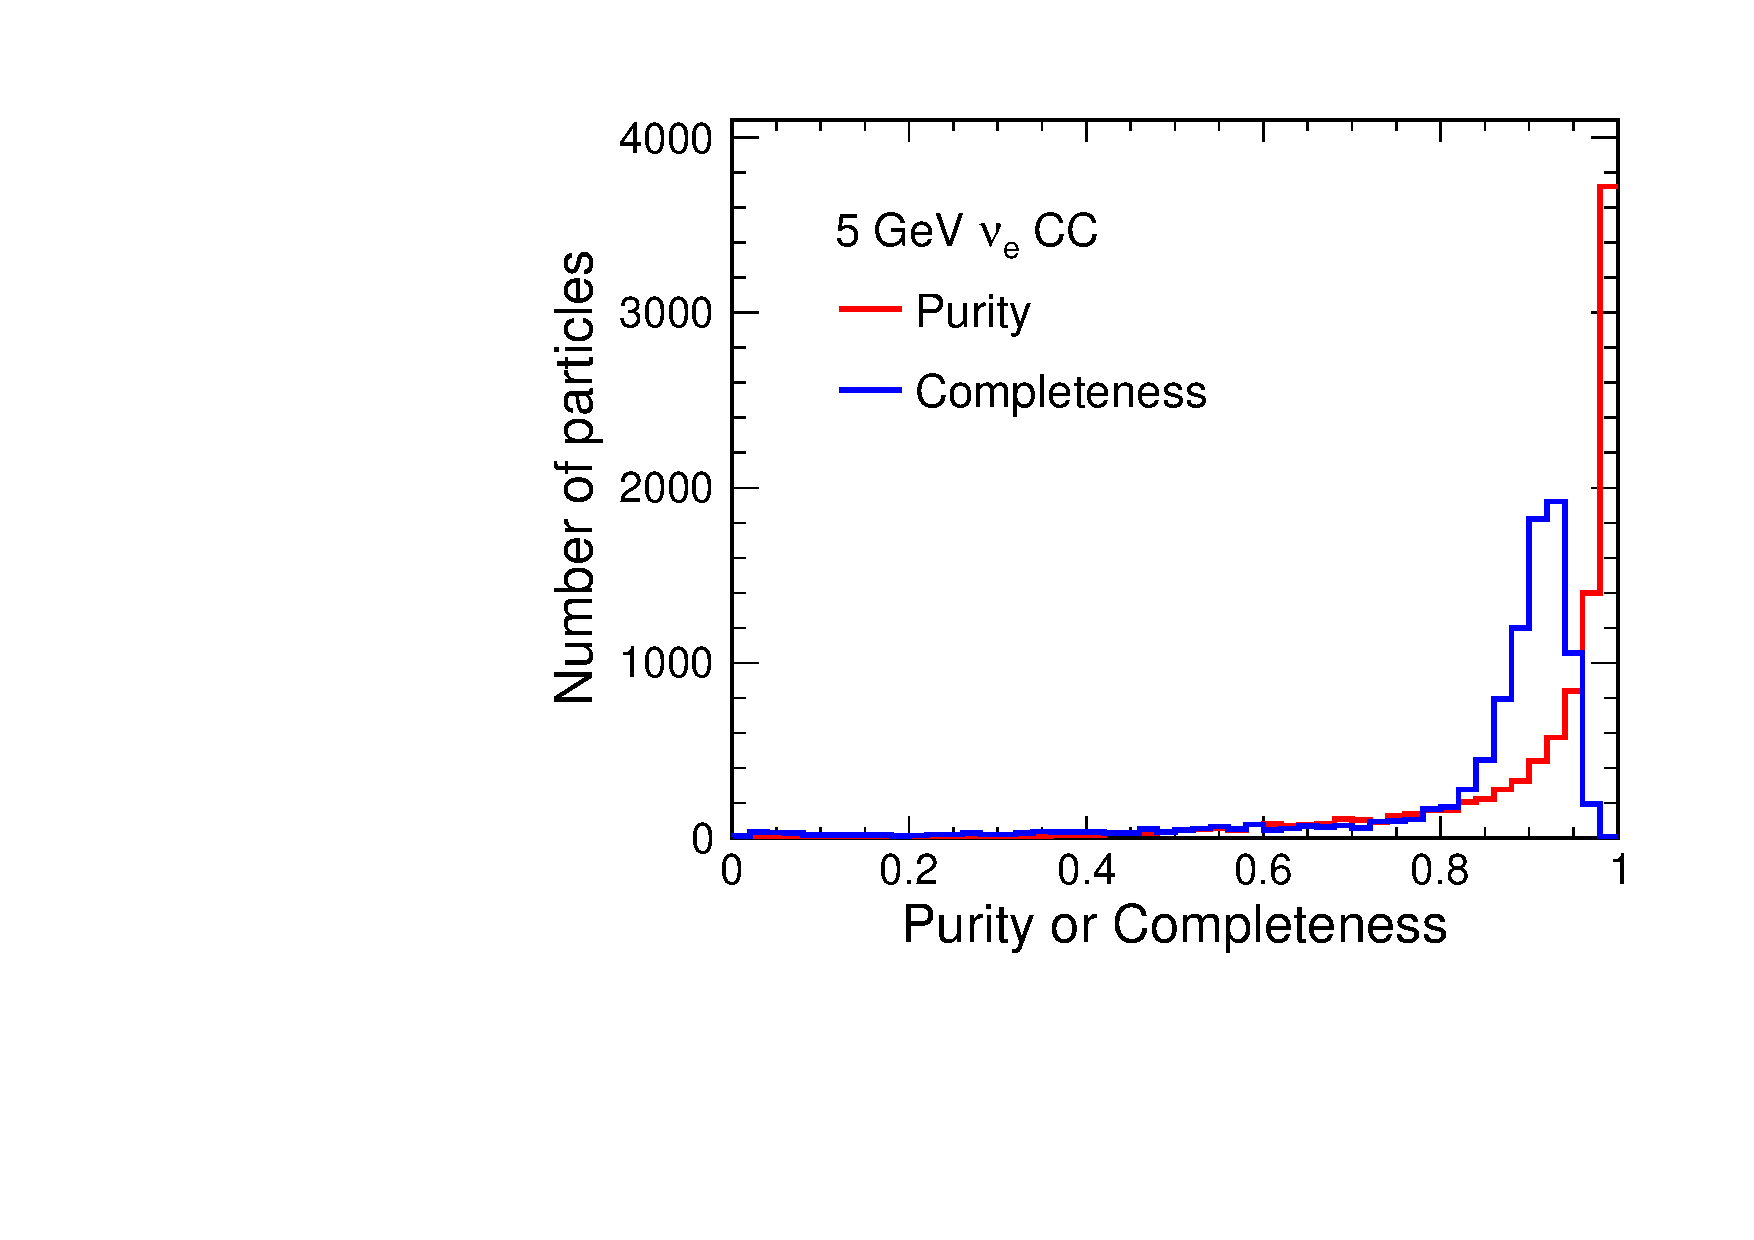
\includegraphics[width=0.49\textwidth]{pandora_uboone_purity_completeness_5GeV_nuecc_annex.pdf}
\end{cdrfigure}

\begin{cdrfigure}[PANDORA vertex resolution]{recoannexpandoravertexresolution}
{Distribution of 2D residuals between reconstructed and simulated interaction
 vertex for 5\,GeV $\nu_{\mu}$ CC (left) and$\nu_{e}$ CC (right) interactions in the MicroBooNE detector.
 The $x$ axis is oriented along the drift field, the $y$ axis runs parallel 
 to the collection plane wires, and the $z$ axis points along the beam direction.}
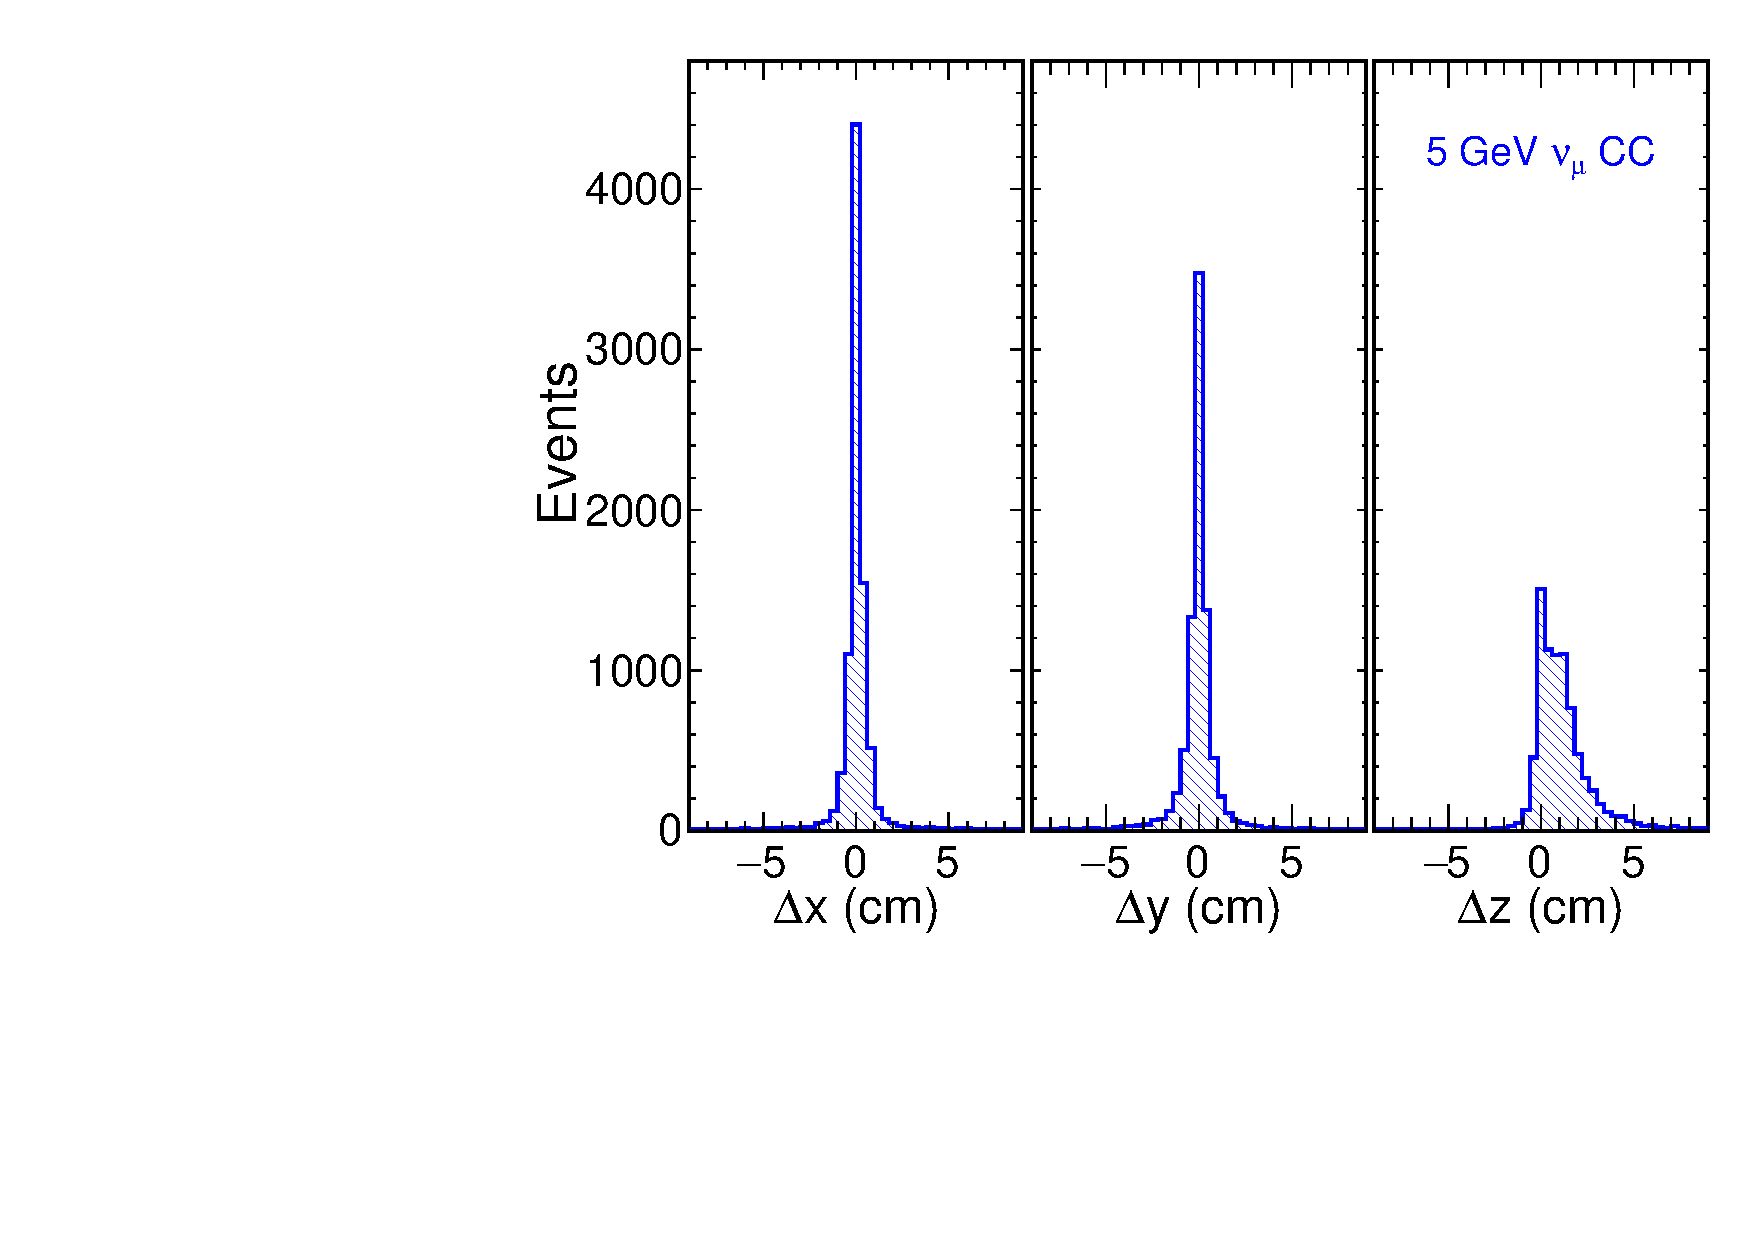
\includegraphics[width=0.49\textwidth]{pandora_uboone_vertex_resolution_numucc_annex.pdf}
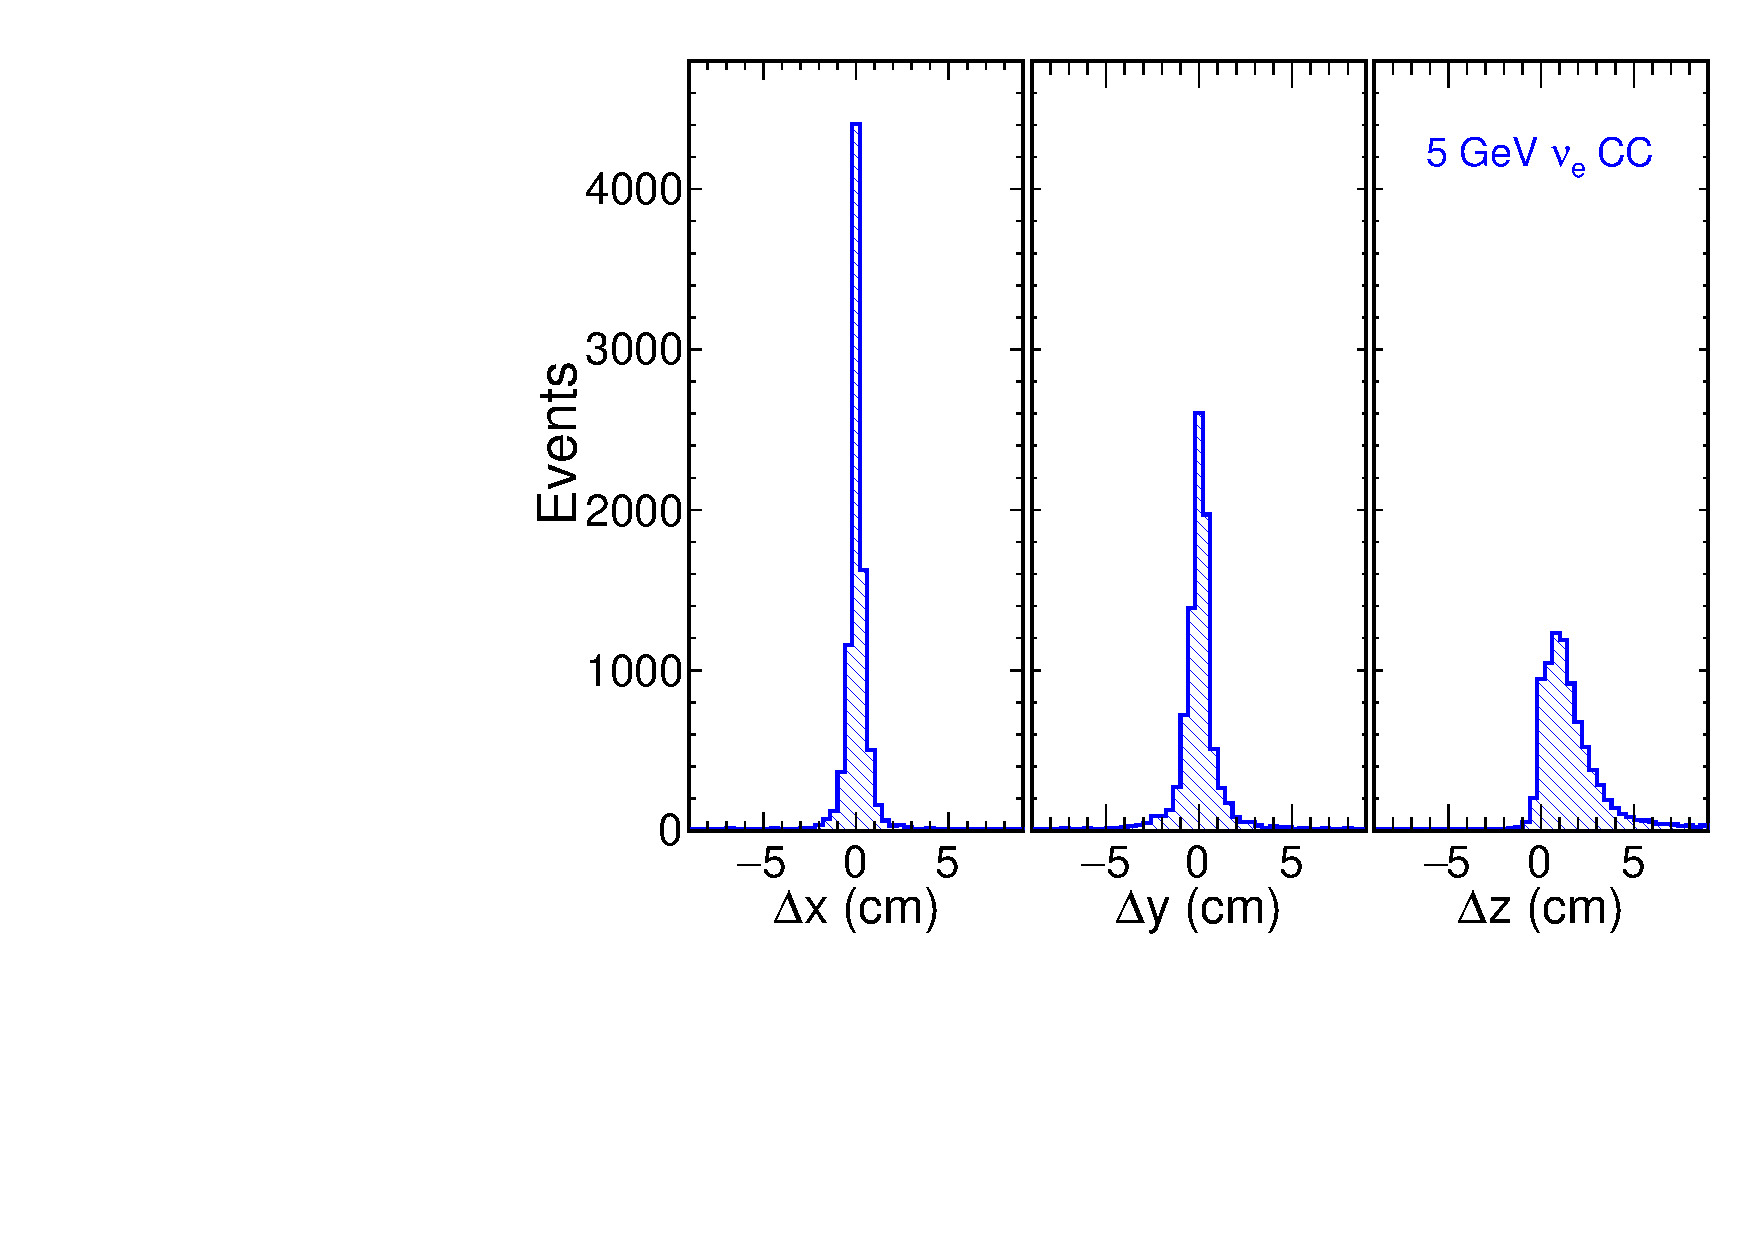
\includegraphics[width=0.49\textwidth]{pandora_uboone_vertex_resolution_nuecc_annex.pdf}
\end{cdrfigure}


\subsection{Track Fitting}

%%%%% Section taken from the LArSoft NIM article -- to rephrase

The track reconstruction problem in a liquid argon TPC is divided
into: trajectory reconstruction, and track parameter estimation.
Hits are the input data for track reconstruction. Hits represent a
one-dimensional measurement of a track (the drift time) on a
measurement surface defined by the charge drift direction and the
readout wire. Hits from multiple views may be combined into
three-dimensional space points. Three dimensional track reconstruction
can proceed from space points or directly from hits.

The Kalman filter algorithm~\cite{kalman} has been widely used in high
energy physics for track reconstruction. The Kalman filter provides an
elegant mathematical solution to the problem of finding an optimal
track description from a collection of candidate measurements that are
hits or space points, especially in cases where the number of
measurements is much larger than the five parameters needed to specify
a track on a surface.  The Kalman filter can be used for both pattern
recognition and parameter estimation.


\fixme{Some text from the main CDR section...}

The three-dimensional reconstruction of tracks can proceed either 
directly from 2D hits or via 3D space points, 
calculated by matching 2D clusters between views.

The well-established Kalman filter technique~\cite{kalman} has been applied
to 3D track reconstruction by both ICARUS~\cite{REF1} and ArgoNeuT~\cite{REF2}.
This technique incorporates the effects of multiple Coulomb scattering,
enabling a scattering-based estimate of the track momentum,
which is shown by ICARUS to be as good as $\Delta p/p \approx 10\%$, 
depending mainly on the track length~\cite{REF3}.
The data from ICARUS have also been used to develop a precise
track reconstruction, which builds a 3D trajectory for each track by simultaneously
optimising its 2D projections to match the observed data~\cite{Antonello:2012hu}.
Another promising technique, based on the local principal curve algorithm, 
has been implemented in conjunction with the development of the 
dual-phase detector concept~\cite{REF4}, and is shown to provide 
a precise reconstruction of two-particle event topologies~\cite{REF5}. 

\fixme{Can we say something about current status or performance?}

%%%% MAYBE TOO MUCH DETAIL FOR CDR 

%The measurement surfaces in liquid argon TPCs intersect, which
%means there is no predetermined order in which the measurement
%surfaces should be visited.  To prevent back-and-forth tracking, which
%would overestimate propagation noise, such as multiple Coulomb
%scattering, the LArSoft Kalman filter chooses the measurement
%surfaces associated with one view as primary, and visits these
%surfaces in their natural predetermined order.  Hits from views other
%than the primary view are added to the track by treating the
%propagation from the track surface to the non-parallel hit measurement
%surface as part of the measurement function.  This measurement
%propagation is always done using a linear approximation as is the
%measurement function, and is done without propagation noise.

%The LArSoft Kalman filter does not use a branching track model. Hit
%selection for the LArSoft Kalman filter is implemented such that at
%each measurement surface, the filter accepts either zero or one
%hit. 

%If the Kalman filter assigns the wrong hit to a track, the track may follow
%the wrong road (e.g. a delta ray), or the track may otherwise end
%prematurely.  Fixing broken tracks relies on a track-stitching
%algorithm that runs after the initial Kalman filter reconstruction.

\subsection{Shower Measurement}

%%%%% Section taken from the LArSoft NIM article -- to rephrase

The electromagnetic shower algorithms have two
steps. The first is a post-clustering stage which examines the
existing clusters in terms of their 2D parameters to determine whether
the clusters are shower-like or track-like. 
The selected shower-like clusters are examined to assign starting points,
directions and angles in the wire-time plane. The second step is 
3D shower reconstruction, which
matches the 2D clusters between views in order to obtain 3D shower axes and start points.
These 3D parameters allow the calculation of the shower energies and charge
depositions at the starts of the showers, which are used in particle
identification. 

\fixme{Can we say something about current status or performance?}

\subsection{Calorimetry}

%%%%% Section taken from the LArSoft NIM article -- to rephrase

As charged particles traverse a volume liquid argon, they deposit
energy through ionization and scintillation. It is important to
measure the energy depotion as it provides information on particle
energy and species. The algorithm for reconstructing the ionization
energy in LArSoft is optimized for line-like tracks and is being
extended to showers. 
For each hit on a reconstructed track, the hit area or amplitude, in ADC counts, is
converted to the charge $Q_{\rm{det}}$, in fC units, on the wire using an
ADC to fC conversion factor that is determined by muons or test-stand
measurements. To account for the charge loss along the drift due to
impurities, a first correction is applied to $Q_{\rm{det}}$ to get the free
charge after recombination $Q_{\rm{free}} = Q_{\rm{det}}/e^{-t/\tau_{e}}$, where
$t$ is the electron drift time for the hit and $\tau_{e}$ is the
electron lifetime measured by the muons or purity monitors. The charge
$Q_{\rm{free}}$ is divided by the track pitch $dx$, which is defined as the
dot production of track direction and the direction normal to the wire
direction in the wire plane, to get the $dQ_{\rm{free}}/dx$ for the
hit. Finally, to account for charge loss due to recombination, also
known as ``charge quenching'', a second correction is applied to
convert $dQ_{\rm{free}}/dx$ to $dE/dx$ based on the modified box model
\cite{Thomas:1987zz} or Birks's model\cite{Birks:1964zz}. The total energy
deposition from the track is obtained by summing the $dE/dx$ from each
hit: $\sum\limits_{i}^{\rm{all\ hits}}(dE/dx)_{i}\cdot dx_{i}$.

%first part same for Qscan (quenching, charge loss)
%
%leave what follow commented for the moment
%In the case of double phase LAr TPC events, 
%the energy scale parameters have been estimated, independently of the actual inputs to the Monte Carlo, using particle gun events. 
%Particles were generated at a range of energies, and the
%measured hit energies summed.
%This approach motivated by the fact that energy deposition profiles vary between particle types, the quenching factor, and therefore the energy scale, will be different depending on the c%luster. In principle, the quenching scale should also depend on the particle energy, but this dependence is seen to be small.


\subsection{Particle Identification}

%%%%% Section taken from the LArSoft NIM article -- to rephrase

If the incident particle stops in the LArTPC active volume, the energy
loss, $dE/dx$, as a function of the residual range ($R$), the path
length to the end point of the track, is used as a powerful method for
particle identification. There are two methods in LArSoft to determine
particle species using calorimetric information. The first method
calculates four $\chi^{2}$ values for each track by comparing measured
$dE/dx$ versus $R$ points to the proton, charged kaon, charged pion
and muon hypotheses and identifies the track as the particle that
gives the smallest $\chi^{2}$ value. The second method calculates the
quantity ${\rm{PIDA}} = <A_{i}> = <(dE/dx)_{i}R_{i}^{0.42}>$ \cite{Thomas:1987zz},
which is defined to be the average of $A_{i} =
(dE/dx)_{i}R_{i}^{0.42}$ over all track points where the residual
range $R_{i}$ is less than 30 cm. The particle species can be
determined by making a selection on the PIDA value.

\fixme{Talk about e-gamma separation here}

\subsection{Neutrino Event Reconstruction}

\fixme{Talk about event classification here:}

In Qscan, a multivariate analysis (MVA) was used to separate particle types based on the spatial characteristics of their clusters.
First step performs a principal components analysis (PCA), transforming the axes to lie along the 
cluster direction and perpendicular to it. Several quantities are then calculated to 
characterize the cluster: the lateral spread, the mean charge-weighted inverse distance of hits to the primary cluster axis
(this is expected to distinguish effectively between showers and tracks), the $dE/dx$.
These variables are then fed into Boosted Decision Trees analyses, 
each calculating the signal and background likelihoods for a particular particle hypothesis.
Currently muon, electron, proton and charged pion hypotheses are considered. It is anticipated that these likelihoods will be used in various ways by downstream analysis code, depending on the needs of the specific analysis.
In the present analysis, the BDT results for muon and electron hypotheses are used to identify lepton clusters and classify events. The signal and background distributions for these hypotheses are shown in 
Figure~\ref{fig:recoannexeventclassification}.

The overall performance of the reconstruction chain (from clustering to PID) has been estimated with a simple binned lepton flavor analysis, 
to understand its ability to distinguish $\nu_{e}$ and $\nu_{\mu}$ events.
If a single lepton flavor is identified in the event, then the event is considered as a signal event of the observed lepton flavor. 
If neither or both lepton flavors are identified, the event is discarded.
Numbers of events correctly reconstructed is above 90$\%$ for $\nu_{\mu}$-CCQE events.

%\fixme{Refer to the LAGUNA-LBNO PID plots}


\begin{cdrfigure}[LAGNUA-LBNO event classification]{recoannexeventclassification}
{Plots showing signal and background distributions for electron (a) and muon (b) MVA hypotheses. 
Background consists of all particles not corresponding to the relevant signal type.}
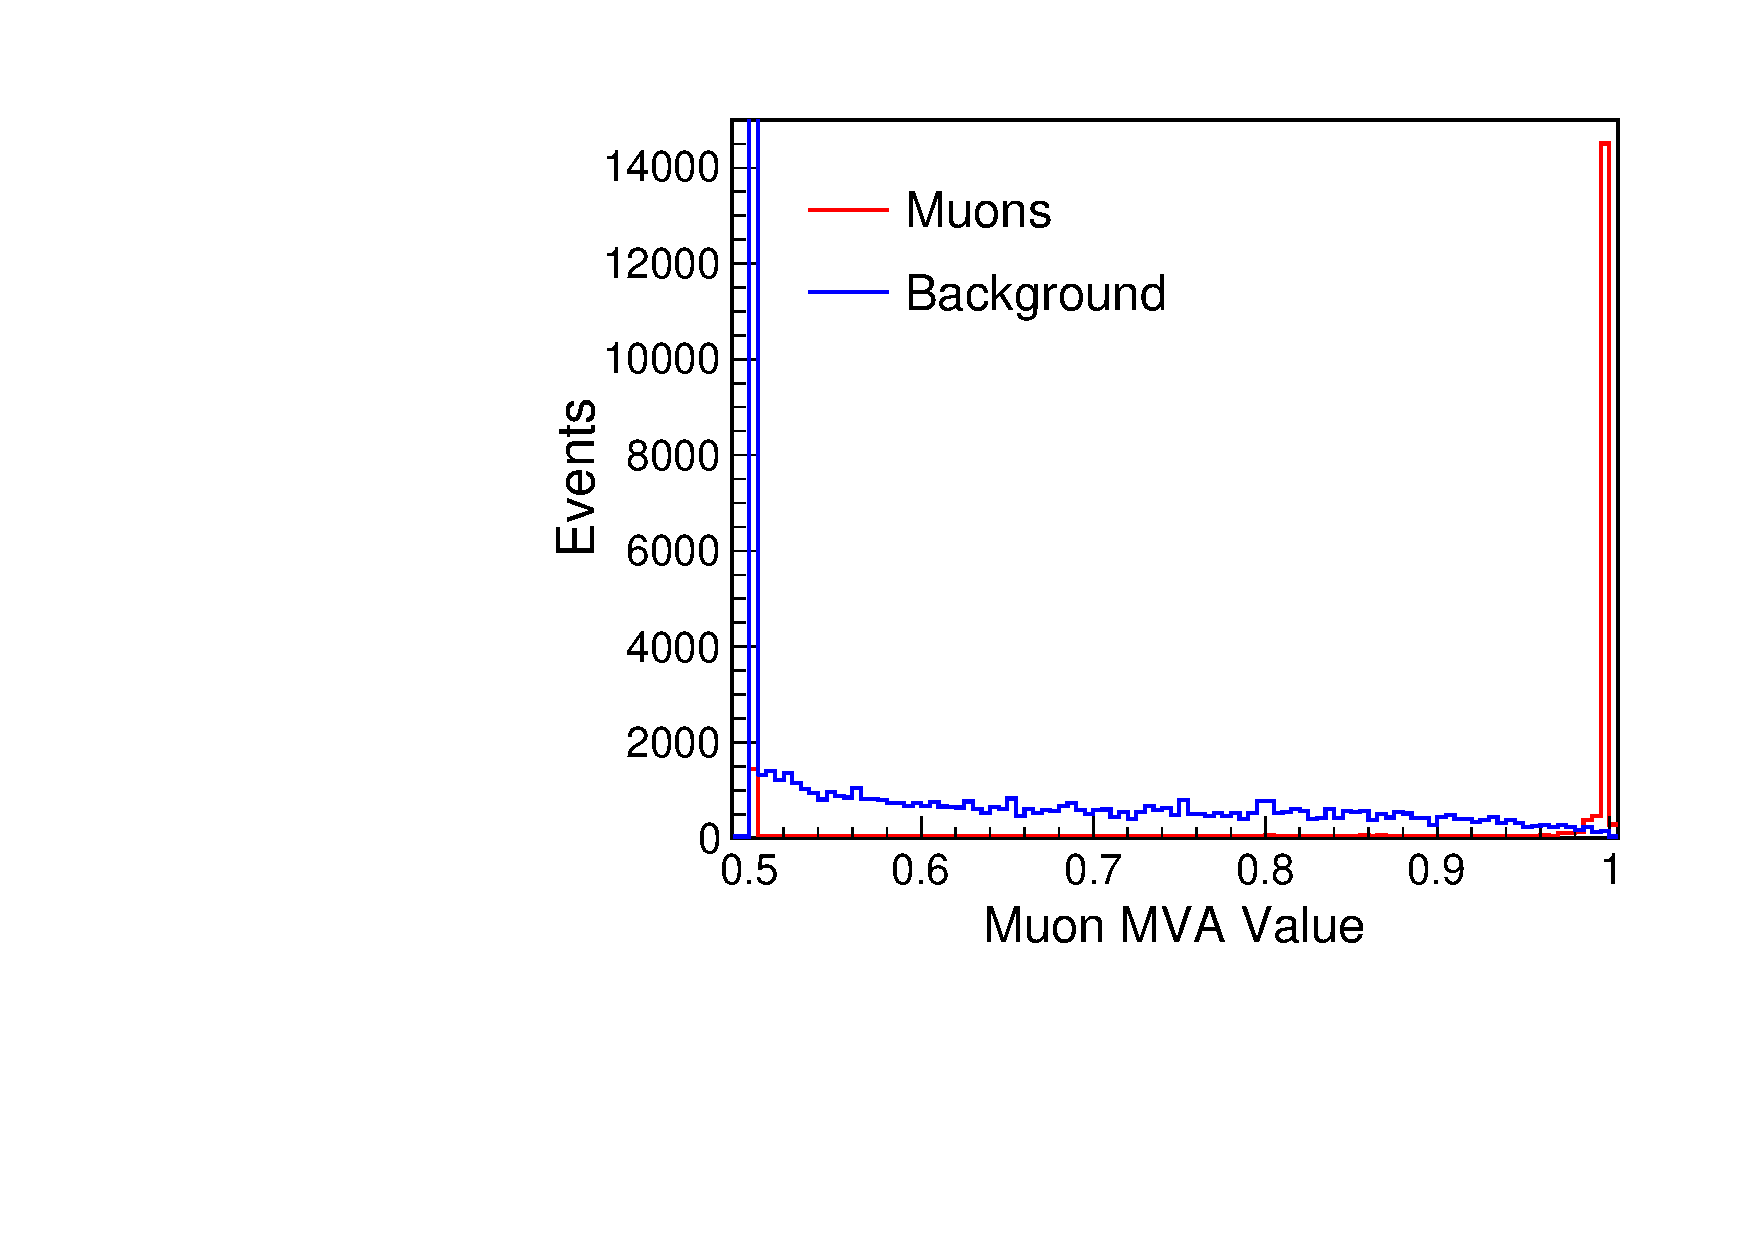
\includegraphics[width=0.49\textwidth]{laguna_lbno_pid_muons.pdf}
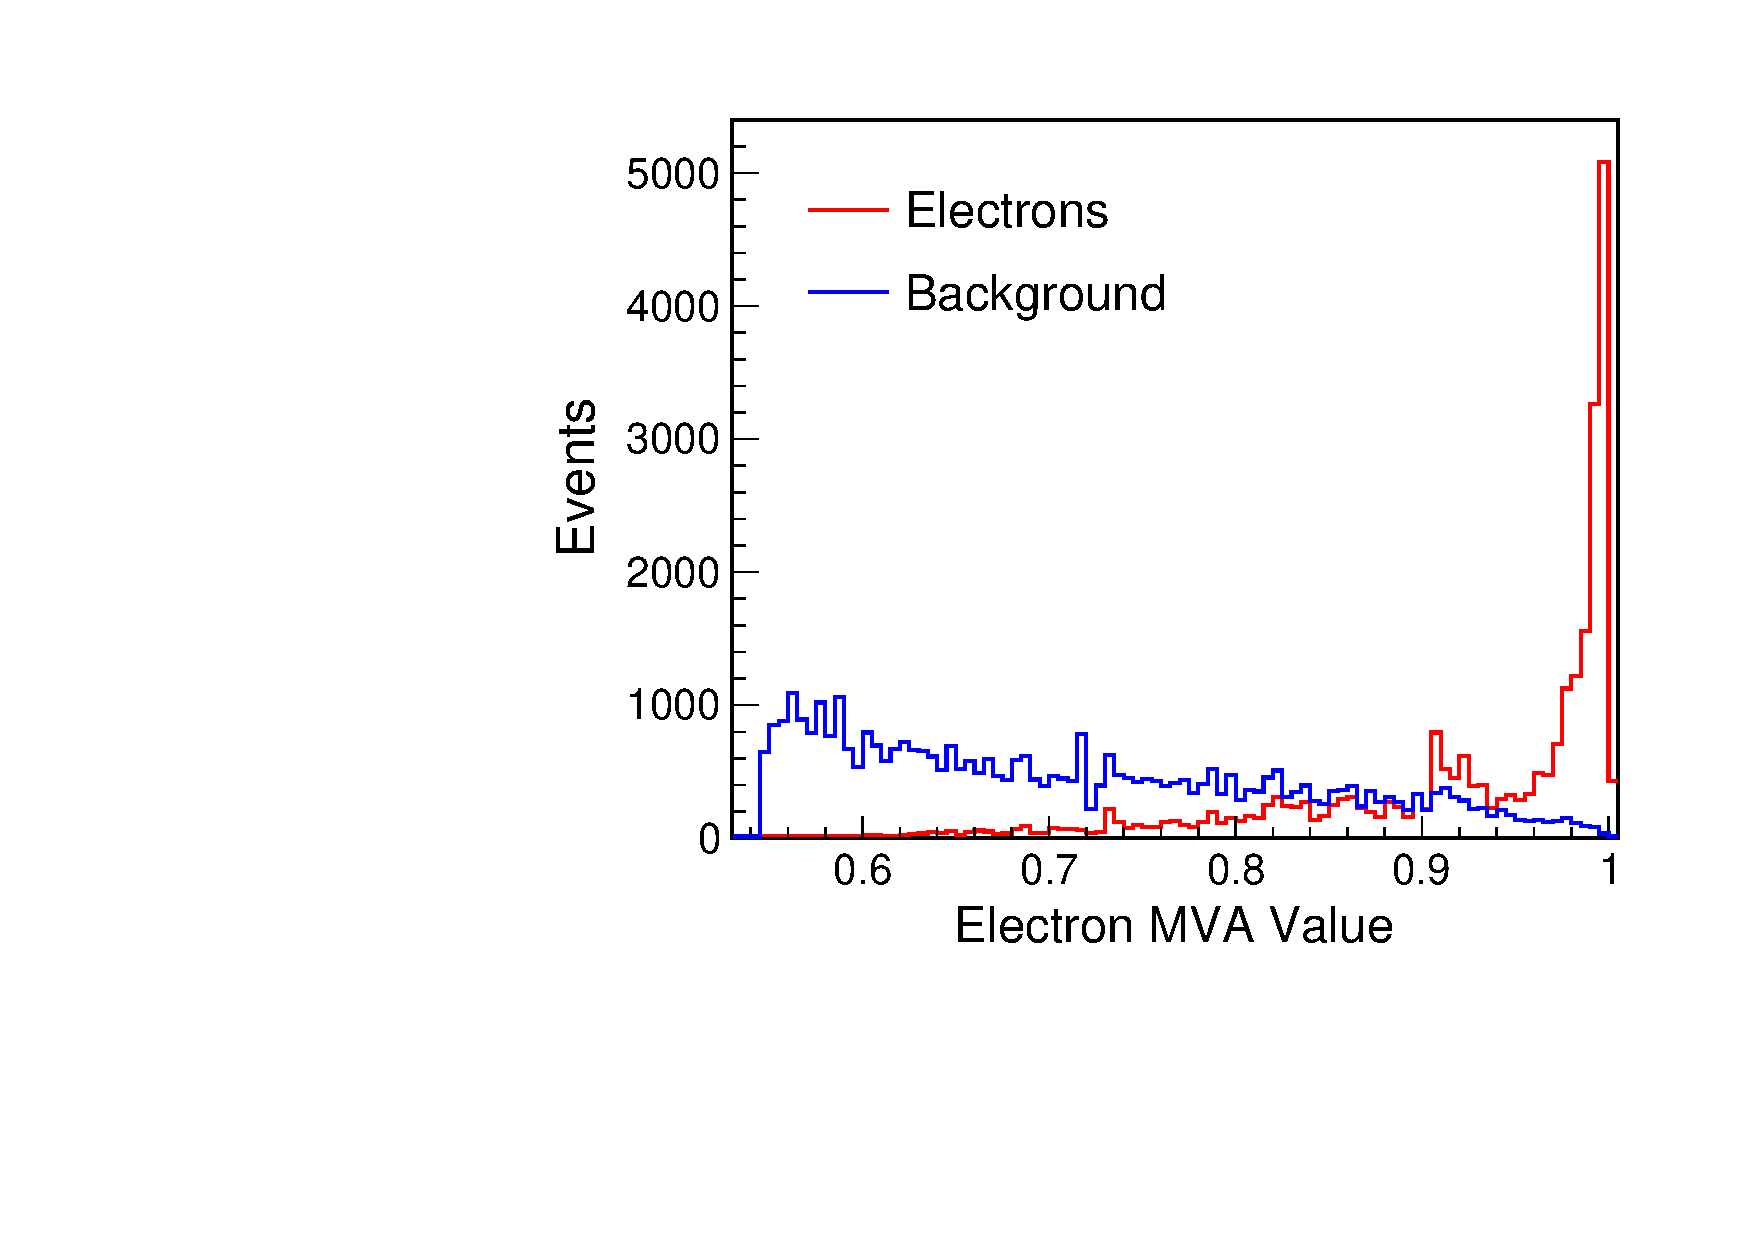
\includegraphics[width=0.49\textwidth]{laguna_lbno_pid_electrons.pdf}
\end{cdrfigure}

%\fixme{Talk about energy reconstruction here:}

For accepted events, the neutrino energy is estimated  assuming a CCQE event and using the two-body approximation, and also calorimetrically.
The calorimetric reconstruction takes account of the quenching factors for the different particles by 
assuming that all hits not associated with the lepton cluster are due to hadronic activity.

It is seen that for high-energy muons, the measured energy saturates. This is due to the muon escaping the detector volume. 


%\fixme{Refer to the LAGUNA-LBNO Energy plots}

Figure~\ref{fig:recoannexrecoenergynue} shows reconstructed energy versus true energy...
Figure~\ref{fig:recoannexrecoenergynumu} shows reconstructed energy versus true energy...

\begin{cdrfigure}[LAGNUA-LBNO electron neutrino energy measurement]{recoannexrecoenergynue}
{Distributions of reconstructed neutrino energy versus true neutrino energy, assuming two-body kinematics. 
Plots shown are for $\nu_{e}$ CCQE (a) and $\nu_{\mu}$ CCQE (b).}
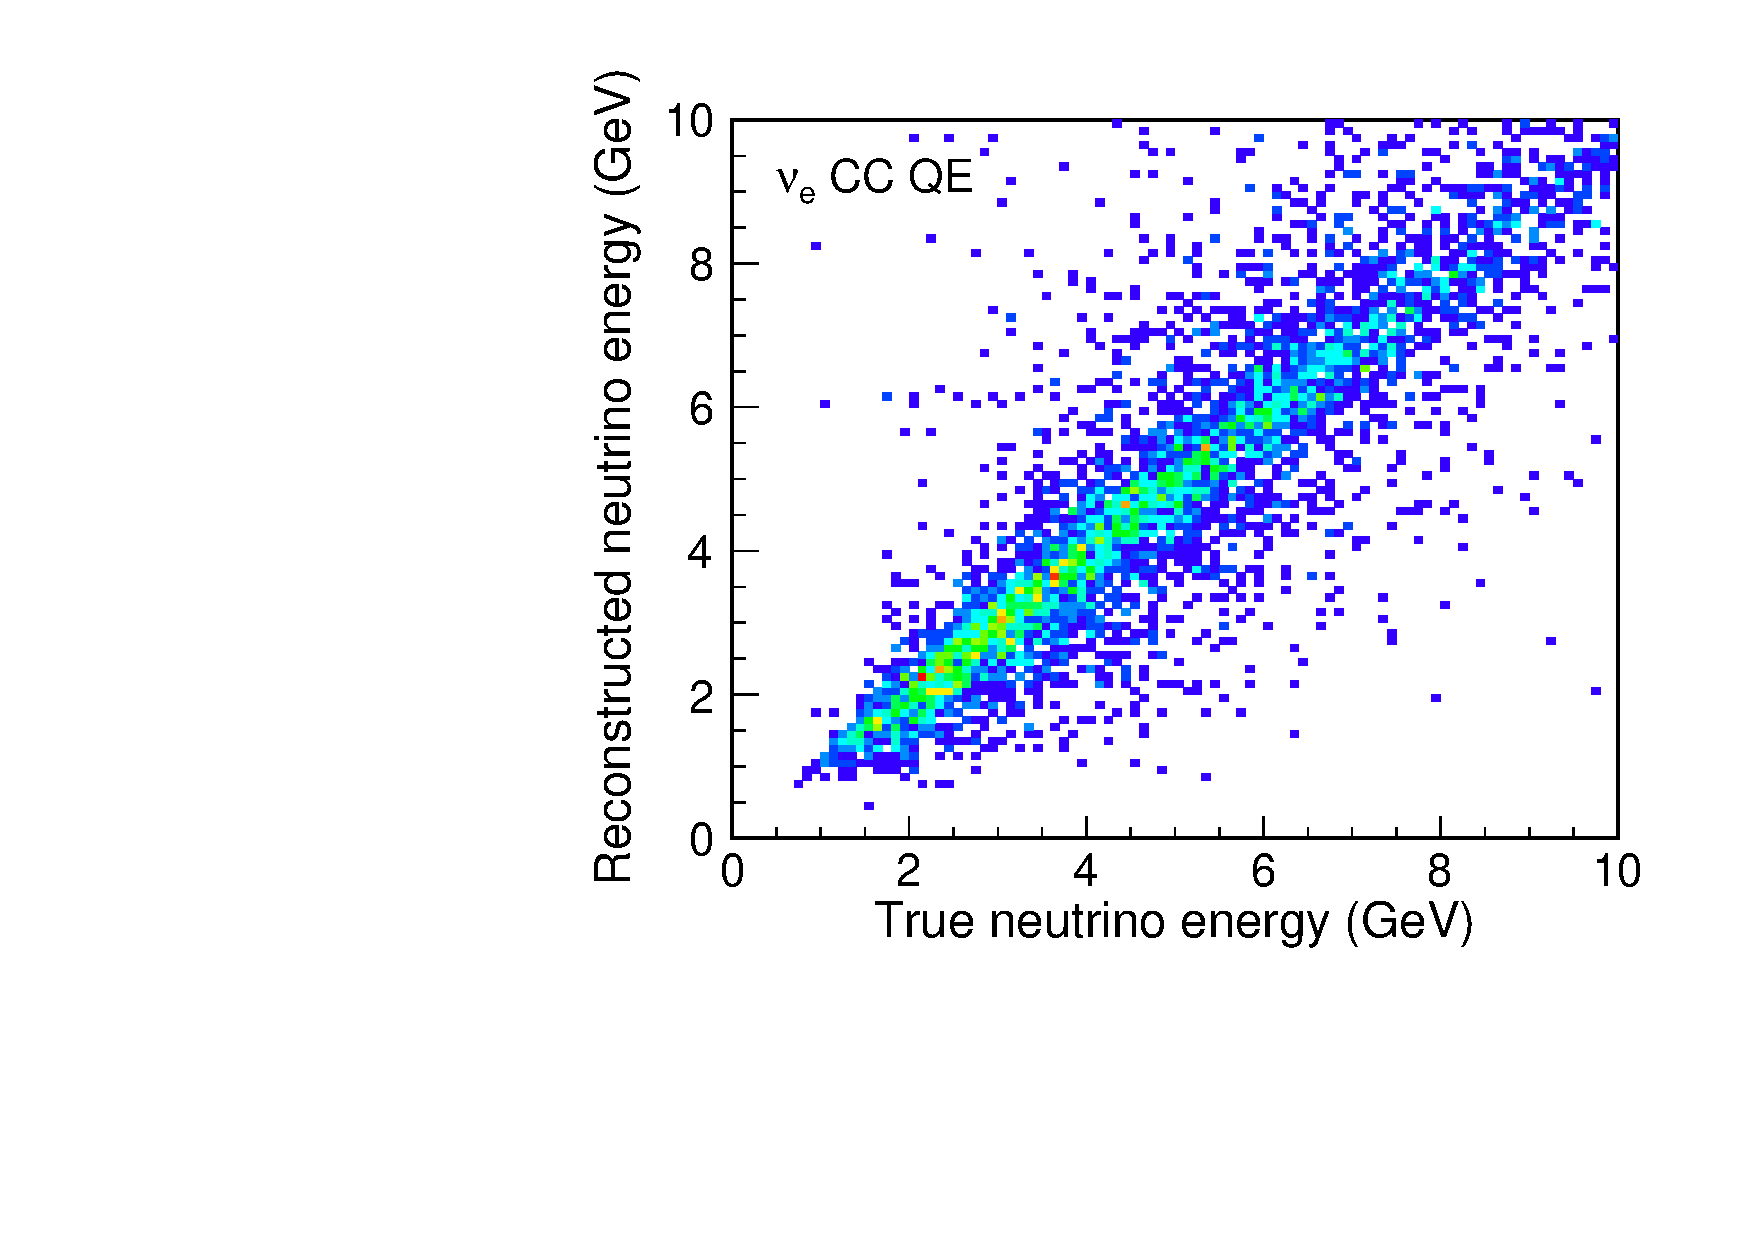
\includegraphics[width=0.49\textwidth]{laguna_lbno_recoenergy_nue_ccqe_annex.pdf}
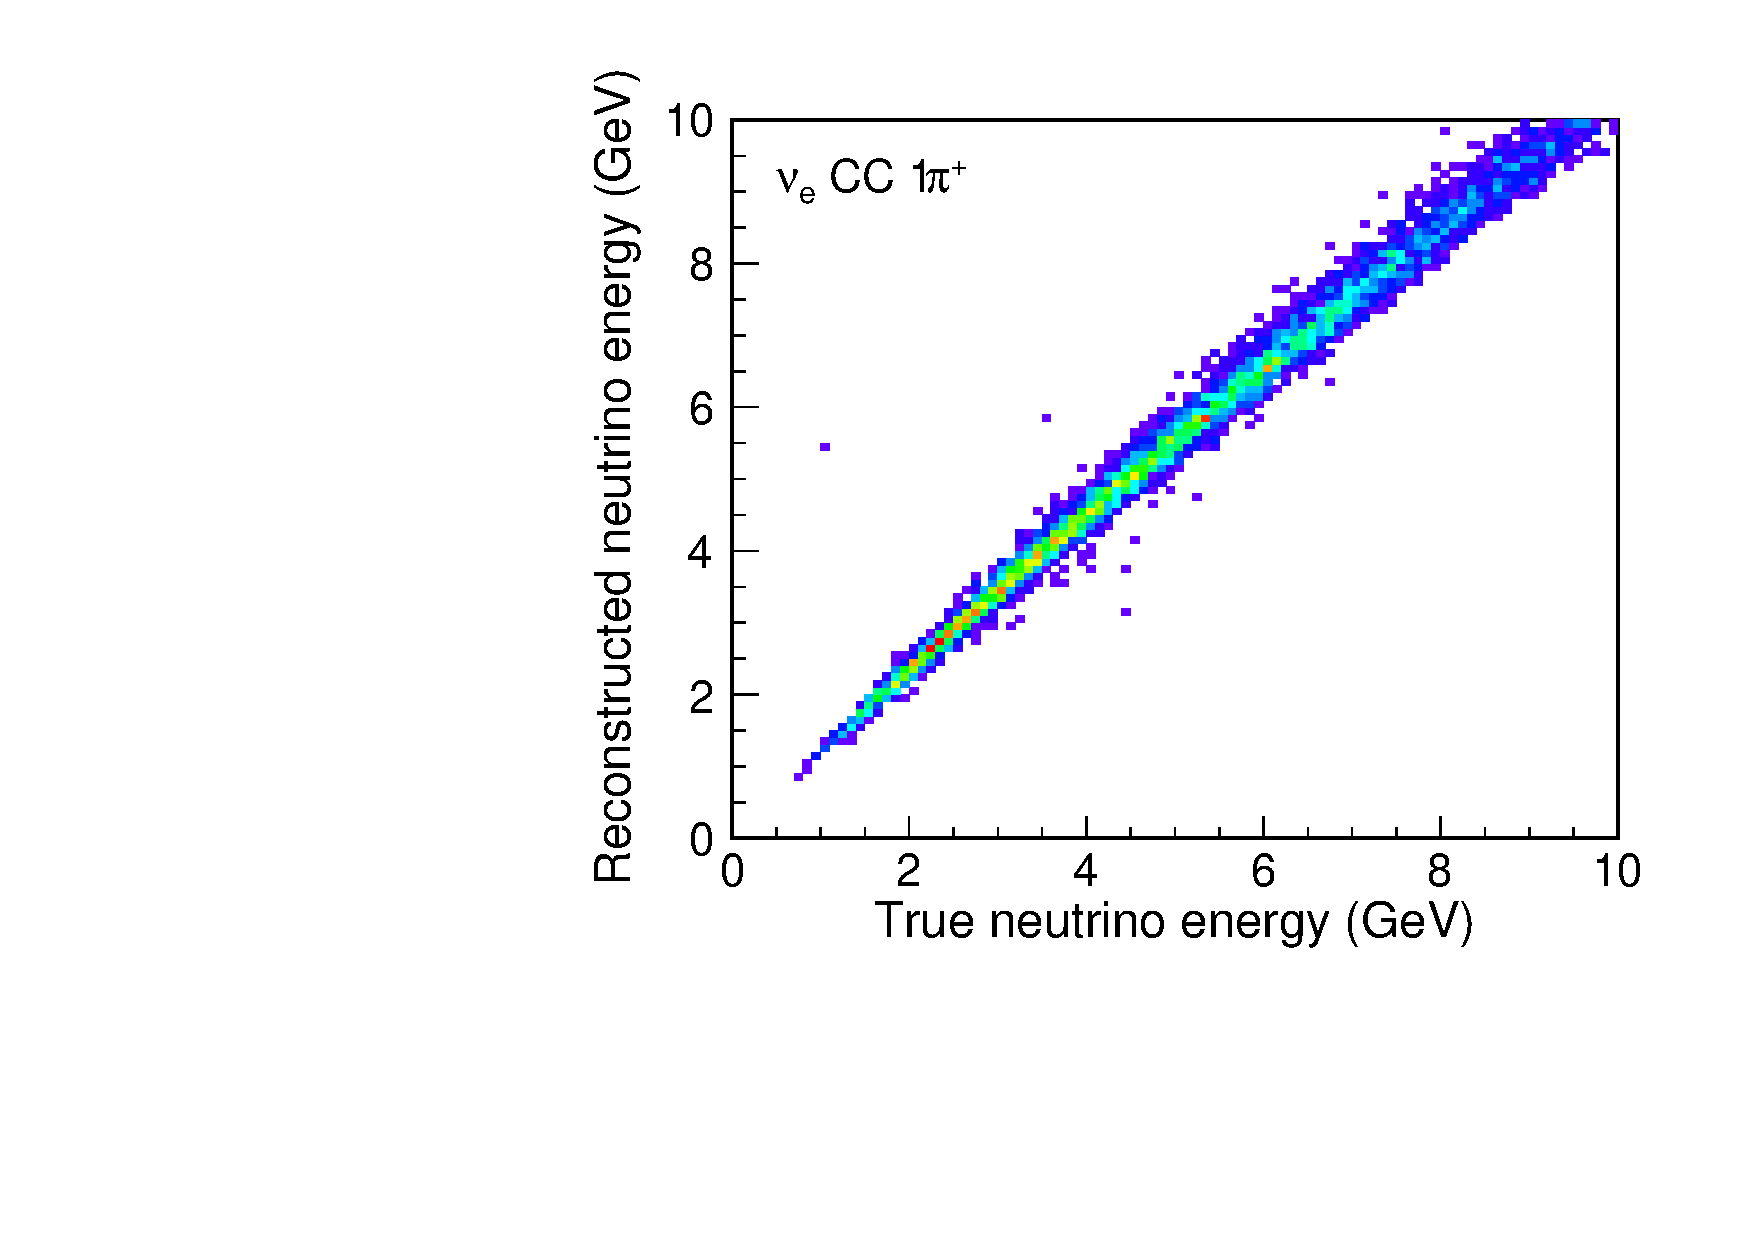
\includegraphics[width=0.49\textwidth]{laguna_lbno_recoenergy_nue_ccres_annex.pdf}
\end{cdrfigure}

\begin{cdrfigure}[LAGNUA-LBNO muon neutrino energy measurement]{recoannexrecoenergynumu}
{Distributions of reconstructed neutrino energy versus true neutrino energy, using calorimetric energy estimation. 
Plots shown are for  $\nu_{e}$  CC1$\pi^{+}$ (a) and $\nu_{\mu}$  CC1$\pi^{+}$ (b).}
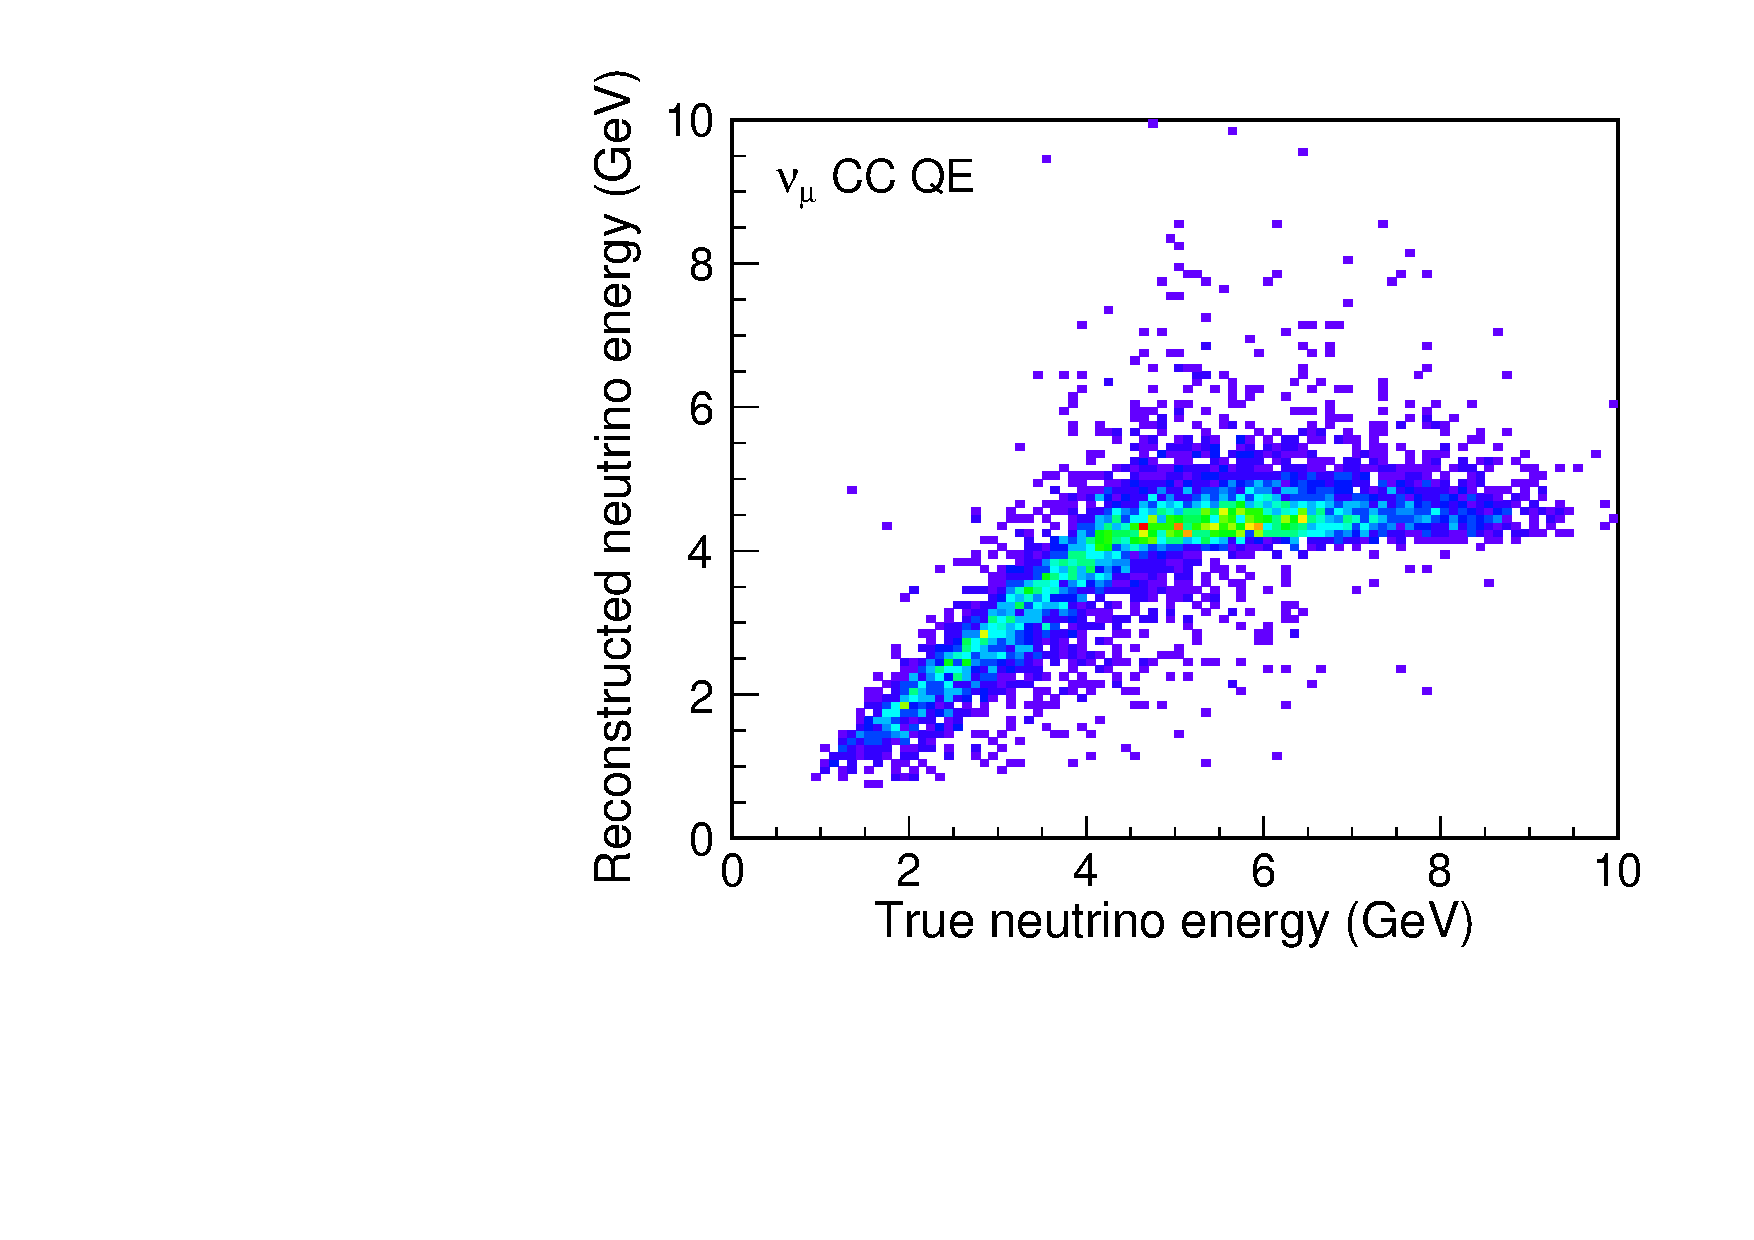
\includegraphics[width=0.49\textwidth]{laguna_lbno_recoenergy_numu_ccqe_annex.pdf}
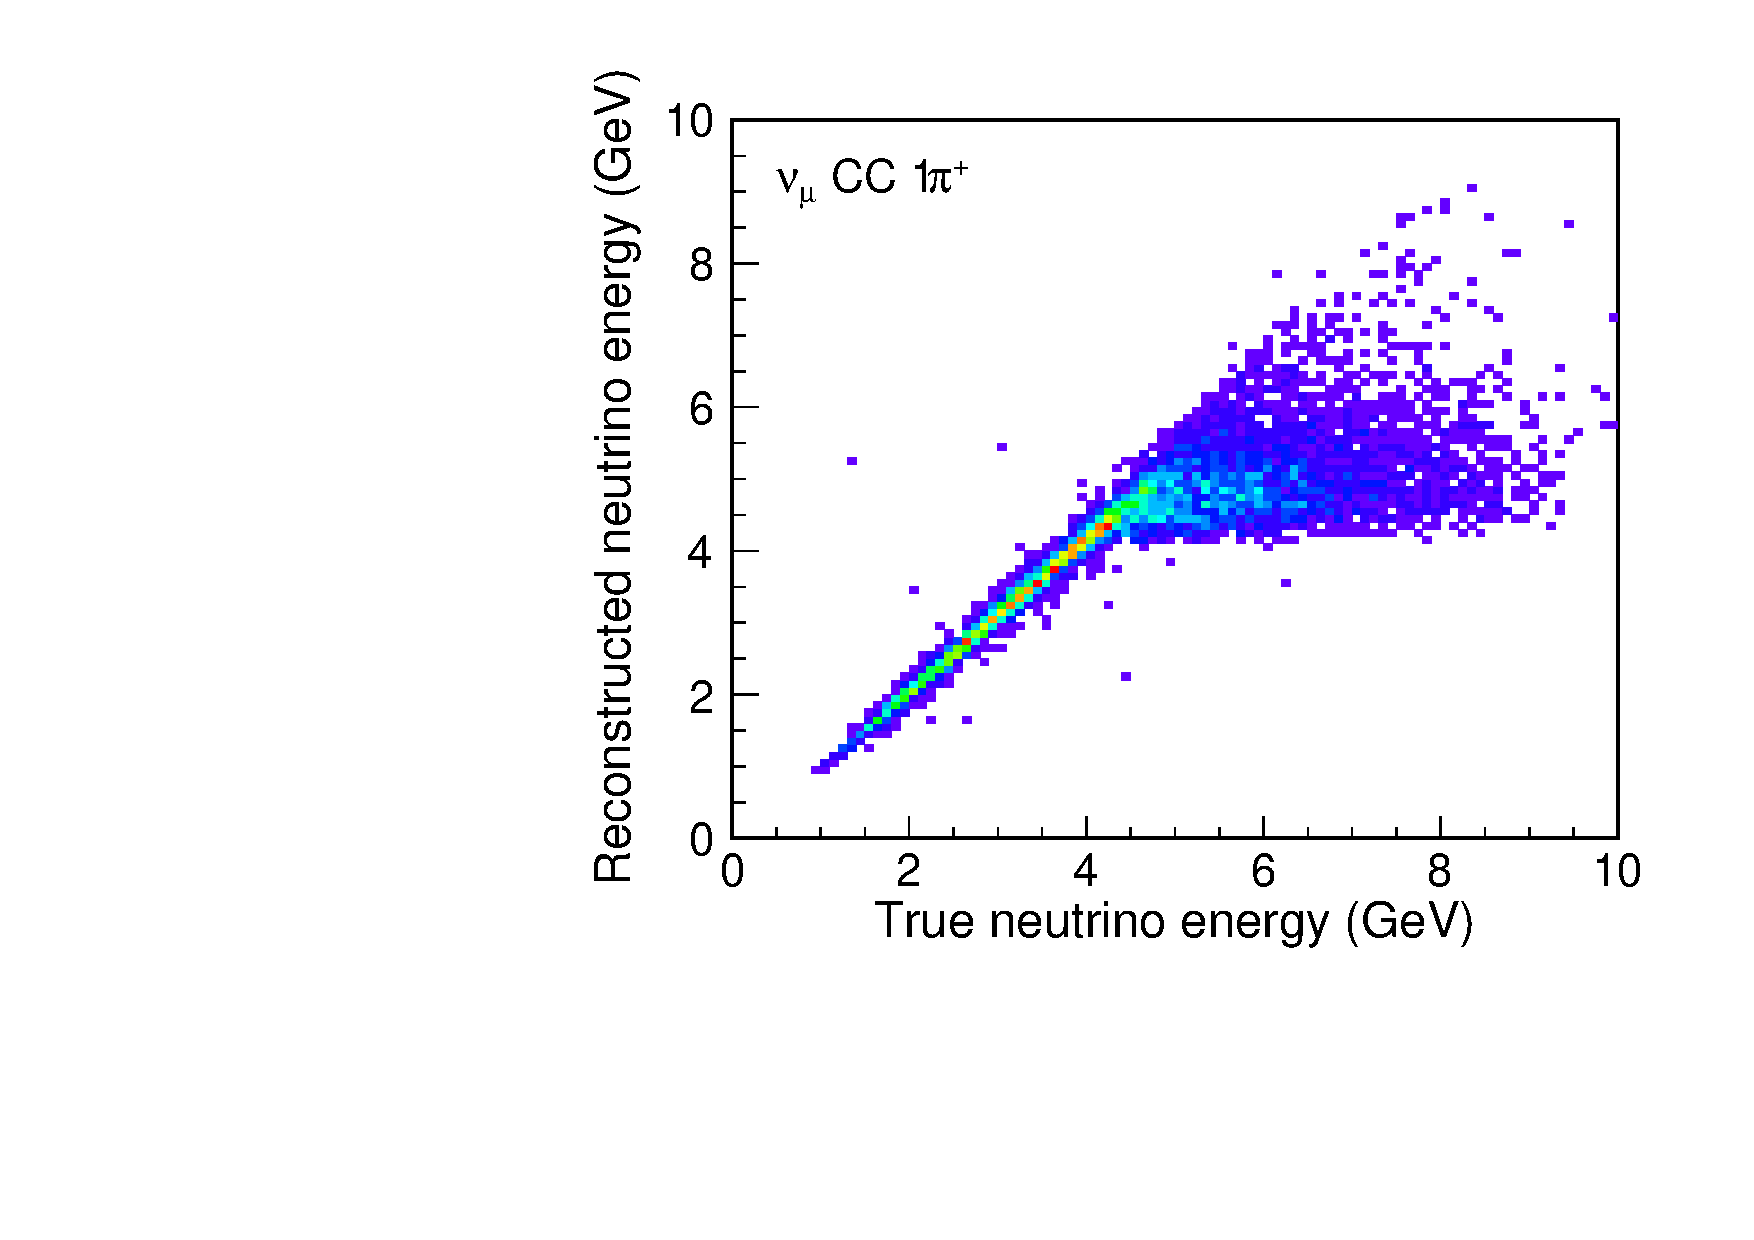
\includegraphics[width=0.49\textwidth]{laguna_lbno_recoenergy_numu_ccres_annex.pdf}
\end{cdrfigure}

%\fixme{Be sure to properly reference LAGUNA-LBNO design study}

\subsection{Calibration}

In order to meet the requirements of high detection efficiency, efficient and
pure particle identification, excellent energy resolution, and small systematic
uncertainties on these performance parameters, calibrations of the detector
will be needed.  {\it In situ} calibration techniques using data collected by the FD
under identical conditions as used for physics analyses are the most desirable.
These include studying cosmic-ray events and non-fiducial interactions.  But not
all performance measures can be calibrated in this way.  A laser calibration system
will constrain the detector alignment as well as measure any residual space-charge effects
(which are expected to be very small underground) and other sources of field non-uniformity,
as well as provide timing calibration and crosscheck the response to drifting charge.  
The electronics will be outfitted with
charge-injection calibration systems so that non-uniformities in the electronics response
can be corrected in a time-dependent fashion.  The response to charged particles of known
energy and particle type will rely on test-beam data from LArIAT and the CERN test
experiments \cernsingleproto{} and \cerndualproto.
